%% LaTeX2e class for student theses
%% thesis.tex
%% 
%% Based on SDQ KIT Template by Erik Burger
%%
%% Karlsruhe Institute of Technology
%% Institute for Automation and Applied Informatics
%% AIDA Research Group
%%
%% Nicole Ludwig
%% nicole.ludwig@kit.edu
%%
%% Version 1.3, 20.11.2018

%% Available page modes: oneside, twoside
%% Available languages: english, ngerman
%% Available modes: draft, final
\documentclass[twoside, english, draft]{thesisIAI}

%% ---------------------------------
%% | Additonal Packages |
%% ---------------------------------

\newcommand{\R}{\mathbb{R}}
\renewcommand{\P}{\mathbb{P}}
\newcommand{\set}[1]{\{#1\}}

\usepackage{tikz}
\usetikzlibrary{shapes}
\usetikzlibrary{plotmarks}
\usetikzlibrary{fit}
\usetikzlibrary{overlay-beamer-styles}
\usetikzlibrary{positioning}
\usetikzlibrary{calc}
\usetikzlibrary{decorations.pathreplacing}
\usetikzlibrary{decorations.pathmorphing}
\definecolor{lightblue}{RGB}{189,216,238}

\usepackage{etoolbox}
\newcommand{\R}{\mathbb{R}}

\newcommand{\set}[1]{\{#1\}}
\newcommand{\func}[3]{#1\colon #2 \rightarrow #3}

\DeclareMathOperator{\CRPS}{CRPS}

%% ---------------------------------
%% | Information about the thesis  |
%% ---------------------------------

%% Name of the author
\author{Pavel Zwerschke}

%% Title (and possibly subtitle) of the thesis
\title{Nonparametric Distributional Regression Models for Probabilistic Energy Forecasting}

%% Type of the thesis 
%\thesistype{Master's Thesis}
\thesistype{Bachelor's Thesis}
%\thesistype{Seminar Paper}

%% Change the faculty here
%\faculty{Seminar}
%\faculty{Engineering}
\faculty{Informatics}
%\faculty{Economics}

%% The advisors are PhDs or Postdocs
\advisorone{Advisor One}
%% The second advisor can be omitted
\advisortwo{Advisor Two}

%% Please enter the start end end time of your thesis
\editingtime{Start Date}{End Date}

\settitle

%% Please do not change anything in this tex file without talking to your supervisor
%% LaTeX2e class for student theses
%% format.tex
%% 
%% Based on SDQ KIT Template by Erik Burger
%%
%% Karlsruhe Institute of Technology
%% Institute for Automation and Applied Informatics
%% AIDA Research Group
%%
%% Nicole Ludwig
%% nicole.ludwig@kit.edu
%%
%% Version 1.2.1, 2018-10-11

%% This file switches between the official reviewers and addresses of the faculties 

\ifthenelse{\equal{\thefaculty}{Seminar}}{\uppertitleback}{
	\ifthenelse{\equal{\thefaculty}{Engineering}}{\uppertitleback{Karlsruher Institut für Technologie\\ Fakultät für Maschinenbau\\ Postfach 6980\\ 76128 Karlsruhe}}{
		\ifthenelse{\equal{\thefaculty}{Informatics}}{\uppertitleback{Karlsruher Institut für Technologie\\ Fakultät für Informatik\\ Postfach 6980\\ 76128 Karlsruhe}}{\uppertitleback{Karlsruher Institut für Technologie \\ Fakultät für Wirtschaftswissenschaften \\ Kollegiengebäude am Kronenplatz \\ Geb. 05.20, 3. OG, Raum 3C-05 \\ 76133 Karlsruhe}}}}

\ifthenelse{\equal{\thefaculty}{Informatics}}{\reviewerone{Prof. Dr. Veit Hagenmeyer}}{\reviewerone{apl. Prof. Dr. Ralf Mikut}}

\ifthenelse{\equal{\thefaculty}{Seminar}}{\reviewertwo{}}{
	\ifthenelse{\equal{\thefaculty}{Informatics}}{\reviewertwo{Prof. Dr. Achim Streit}}{
		\ifthenelse{\equal{\thefaculty}{Engineering}}{\reviewertwo{Prof. Dr. Veit Hagenmeyer}}{\reviewertwo{Prof. Dr. Wolf Fichtner}}}}

\ifthenelse{\equal{\thefaculty}{Seminar}}{\facultyname{Energy Informatics Seminar}}{
	\ifthenelse{\equal{\thefaculty}{Engineering}}{\facultyname{\iflanguage{english}{at the Department of Mechanical Engineering}{an der Fakultät für Maschinenbau}}}{
		\ifthenelse{\equal{\thefaculty}{Informatics}}{\facultyname{\iflanguage{english}{at the Department of Informatics}{an der Fakultät für Informatik}}}{
		\facultyname{\iflanguage{english}{at the Department of Economics and Management}{an der Fakultät für Wirtschaftswissenschaften}}}}}
		
		
		




%% --------------------------------
%% | Settings for word separation |
%% --------------------------------

%% Describe separation hints here.
%% For more details, see 
%% http://en.wikibooks.org/wiki/LaTeX/Text_Formatting#Hyphenation
\hyphenation{
% me-ta-mo-del
}

%% --------------------------------
%% | Bibliography                 |
%% --------------------------------

% Please make sure your bibfiles name is thesis.bib and is located in the tex subfolder
\usepackage[                 % !! what about the ``biblatex.cfg''?
        backend=bibtex8,      % (bibtex), bibtex8, biber
%        %
        style=authoryear,		 %numeric-comp,
%        bibstyle=,          % should not be used without citestyle and vice versa
%        citestyle=,
%        natbib=true,
        %
%        sorting=nty,        % (nty), nyt, nyvt, anty, anyt, anyvt, debug, none
%        sortlos=los,        % bib, (los)
%        sortcites=false,    % false
%        maxnames=2,         % <integer> (3)
				maxcitenames=2,      % sets the maximum numbers of authors before abbreviated to et al in text
				maxbibnames=25,       % sets the maximum numbers of authors before abbreviated to et al in bibliography
%        minnames=1,         % (1)
%        maxitems=3,         % (3)
%        minitems=1,         % (1)
%        autocite=,          % inline, footnote, superscript, ...
%        autopunct=true,     % true
%        babel=none,         % (none), hyphen, other, other*
%        block=none,         % (none), space, par, nbpar, ragged
        hyperref=true,      % false
%        backref=false,      % false
%        indexing=false,     % true, (false), cite, bib
%        refsection=none,    % (none), part, chapter, section, subsection
%        refsegment=none,    % (none), part, chapter, section, subsection
%        citereset=none,     % (none), part, chapter, section, subsection
%        abbreviate=true,    % true
%        date=long,          % short, (long)
%        urldate=short,      % (short), long
%        defernums=false,    % false
%        punctfont=false,    % false
        %
%        mincrossrefs=2,     % 2
        bibencoding=inputenc,   % (ascii), inputenc, <encoding>
        %%
%        keywsort=false,     % false
    %
%     useauthor=false,   % true
%     useeditor=false,   % true
%        useprefix=true,     % false
    %
%        pagetracker=true,   % true, (false), page, spread
%     citetracker=true,   % true, (false), context, strict, constrict
%     ibidtracker=true,   % true, (false), context, strict, constrict
%     opcittracker=true,   % true, (false), context, strict, constrict
%     loccittracker=true, % true, (false), context, strict, constrict
%        terseinits=true,    % false
%     labelalpha=true,   % false
%     labelnumber=true,   % false
%     labelyear=true,   % false
%     singletitle=true,   % false
      uniquename=init,   % true, (false), init
%
        doi=false,
        url=false,
				isbn = false,
        giveninits = true % render first/middle names as initals
            ]{biblatex}
	
\makeatletter
\def\blx@maxline{77}
\makeatother
	
	\bibliography{tex/thesis}
   
      %  \DefineBibliographyStrings{ngerman}{%
         %   bibliography     = {Literaturverzeichnis},  % = \bibname
         %   references       = {Literatur},             % = \refname
     %   }
        \defbibnote{alphabetic}{%
            Die Literaturangaben sind alphabetisch nach den Namen
            der Autoren sortiert. Bei mehreren Autoren wird nach
            dem ersten Autor sortiert.\par
            Und mit dem neuen \LPack{biblatex}-Paket funktioniert
            das auch, wie man unschwer erkennen kann.\par\bigskip
        }

% -------------------------------------------------------------------------------------------------
%% declare author names as "last, first".
%% Either for the first author only or for all authors
%\DeclareNameFormat{author}{%
%    \ifthenelse{\value{listcount}=1}
%        {#1%                                            % first author
%            \ifblank{#3}{}{\addcomma\space #3}}
%        {#1%                                            % all the other authors (last, first)
%            \ifblank{#3}{}{\addcomma\space #3}}%
%%        {\ifblank{#3}{}{#3\space}%                      % all the other authors (first last)
%%            #1}%
%    \ifthenelse{\value{listcount}<\value{liststop}}
%        {,\space}
%            {}
%}
%
%%http://projekte.dante.de/DanteFAQ/BiblatexReihenfolgeAutoren
%\DeclareNameFormat{last-first}{%
%  \iffirstinits
%    {\usebibmacro{name:last-first}{#1}{#4}{#5}{#7}}
%    {\usebibmacro{name:last-first}{#1}{#3}{#5}{#7}}%
%  \usebibmacro{name:andothers}}
%\DeclareNameFormat{labelname}{%
%   \ifuseprefix
%     {\usebibmacro{name:last-first}{#1}{#4}{#5}{#8}}
%     {\usebibmacro{name:last-first}{#1}{#4}{#6}{#8}}%
%   \usebibmacro{name:andothers}}

%  \DefineBibliographyStrings{english}{%
%    typeeditor = {{}{}},
%    typeeditors = {{}{}},
%    in = {{}{}},
%    inseries = {{}{}},
%    byeditor = {{}{}}
%  }

%-------------------------------------------------------------------------------------------------

%% http://www.golatex.de/biblatex-anpassen-die-x-te-frage-t4657.html
\renewbibmacro*{journal+issuetitle}{%
  \usebibmacro{journal}%
  \setunit*{\addcomma\space}%
  \iffieldundef{series}
    {}
    {\newunit
     \printfield{series}%
     \setunit{\addcomma\space}}%
  \printfield{volume}%
  \setunit*{\addcomma\space}%
  \printfield{number}%
  \setunit{\addcomma\space}%
  \printfield{eid}%
  \setunit{\addspace}%
  \usebibmacro{issue+date}%
  \setunit{\addcolon\space}%
  \usebibmacro{issue}%
  \newunit}

\DeclareFieldFormat[article]{volume}{\bibstring{jourvol}~#1}
\DeclareFieldFormat[article]{number}{\bibstring{number}~#1} 
%\DeclareFieldFormat[article]{edition}{\bibstring{edition}~#1} 

%% http://mrunix.de/forums/showthread.php?t=67386
\DefineBibliographyStrings{english}{jourvol={Vol\adddot}} 
\DefineBibliographyStrings{english}{number={No\adddot}} 
\DefineBibliographyStrings{english}{edition={Ed\adddot}} 

\AtBeginBibliography{%
  % Setzt die Autoren-Vornamen auf Kapitälchen 
  \renewcommand*{\mkbibnamefirst}{\textsc}
  \renewcommand*{\mkbibnamelast}{\textsc}
  \renewcommand*{\mkbibnameprefix}{\textsc}
  \renewcommand*{\mkbibnameaffix}{\textsc}
  
  %%Doppelpunkt nach Namen, kein Punkt
  %\renewcommand*{\labelnamepunct}{\addcolon\space} 
  
  \DeclareFieldFormat{name}{\textsc{#1\isdot}}
  \DeclareFieldFormat{title}{\mkbibemph{#1\isdot}}
  
  %%\DeclareFieldFormat[article]{title}{#1}
  %%\DeclareFieldFormat[article]{title}{\mkbibquote{#1}}
  \renewcommand*{\mkbibquote}[1]{\mkbibemph{#1\isdot}}
 
  % http://tex.stackexchange.com/ ...
  % questions/16716/spell-out-volume-and-edition-in-words-biblatex-in-german
  %\renewcommand*{\mkbibordedition}[1]{\Ordinalstringnum{#1}[f]}
  \renewcommand*{\mkbibordedition}[1]{\ordinalnum{#1}}
} 
\usepackage[toc]{glossaries}

%\glstoctrue

\newacronym{emos}{EMOS}{Ensemble Model Output Statistics}
\newacronym{ecmwf}{ECMWF}{European Centre for Medium-Range Weather Forecasts}
\newacronym{eps}{EPS}{Ensemble Prediction System}
\newacronym{ecc}{ECC}{Ensemble Copula Coupling}
\newacronym{pdf}{PDF}{Probability Distribution Function}
\newacronym{nwp}{NWP}{Numerical Weather Prediction}
\newacronym{crps}{CRPS}{Continuous Ranked Probability Score}
\newacronym{mape}{MAPE}{Mean Absolute Percentage Error}
\newacronym{rmse}{RMSE}{Root Mean Squared Error}


%\renewcommand{\glsnamefont}[1]{\emph{#1}}
\setlength{\glsdescwidth}{0.9\linewidth}

\makeglossaries

%% ====================================
%% ====================================
%% ||                                ||
%% || Beginning of the main document ||
%% ||                                ||
%% ====================================
%% ====================================

%% Set PDF metadata
\setpdf

\begin{document}

\hypersetup{pageanchor=false}

%% Set the title
\maketitle

%% The Preamble begins here
\frontmatter

%% LaTeX2e class for student theses: Declaration of independent work
%% sections/declaration.tex
%% 
%% Karlsruhe Institute of Technology
%% Institute for Program Structures and Data Organization
%% Chair for Software Design and Quality (SDQ)
%%
%% Dr.-Ing. Erik Burger
%% burger@kit.edu
%%
%% Version 1.3.2, 2017-08-01

\thispagestyle{empty}
\null\vfill
\noindent\hbox to \textwidth{\hrulefill} 
\iflanguage{english}{I declare that I have developed and written the enclosed
\ifthenelse{\equal{\thefaculty}{Engineering}}{thesis}{\ifthenelse{\equal{\thefaculty}{Informatics}}{thesis}{paper}} completely by myself, and have not used sources or means without
declaration in the text.}%
{Ich versichere wahrheitsgemäß, die Arbeit
selbstständig angefertigt, alle benutzten Hilfsmittel vollständig und genau
angegeben und alles kenntlich gemacht zu haben, was aus Arbeiten anderer
unverändert oder mit Änderungen entnommen wurde.}
 
 
%% ---------------------------------------------
%% | Replace PLACE and DATE with actual values |
%% ---------------------------------------------
\textbf{PLACE, DATE}
\vspace{1.5cm}
 
\dotfill\hspace*{8.0cm}\\
\hspace*{2cm}(\theauthor) 
\cleardoublepage

\setcounter{page}{1}
\pagenumbering{roman}

%% ----------------
%% |   Abstract   |
%% ----------------
 
%% For theses written in English, an abstract both in English
%% and German is mandatory.
%%
%% Seminar Papers written in English need only an English abstract.
%%
%% For theses written in German, a German abstract is sufficient.
%%
%% The text is included from the following files:
%% - sections/abstract
%% - sections/zusammenfassung

\pdfbookmark[1]{Abstract}{Abstract}

\chapter*{Abstract}

\begin{center}
  \begin{minipage}{12cm}
    \begin{sloppypar}
      As the share of electricity from regenerative sources is growing constantly, 
      it makes sense to predict the power generation of these sources. 
      In order to model the uncertainty of a forecast, one often predicts the probability 
      distribution of the corresponding random variable. There are many different nonparametric machine learning approaches 
      to the solar power generation forecasting problem. Hence, this thesis compares three approaches 
      in order to predict solar power generation, namely Quantile Random Forests, Nearest Neighbor Quantile Filters and 
      Spline Quantile Functions RNN. The performance of the models is evaluated on the Global Energy Forecasting Competition 2014 
      dataset. 
      We see that the Quantile Regression Forests manage to get the best score of \(0.01873\) following 
      the Nestest Neighbor Quantile Filters model with a score of \(0.0194\) and the Spline Quantile Functions RNN model with a score of \(0.02041\). 
    \end{sloppypar}
  \end{minipage}
\end{center}

\hypersetup{pageanchor=true}
%% ------------------------
%% |   Table of Contents  |
%% ------------------------
\tableofcontents
\listoffigures
\listoftables

\printglossary[title=Abbreviations, toctitle=List of Abbreviations, 
style=super, nogroupskip, nopostdot, nonumberlist]

%% -----------------
%% |   Main part   |
%% -----------------

\mainmatter

\chapter{Introduction}
\label{ch:Introduction}

\stress{\textbf{Disclaimer to this document:} 
This is a template with some additional thesis information and a sample structure. 
The structure includes the chapters most commonly needed in a thesis. 
Neither the order nor the chapter titles are fixed and will most likely 
have to be adapted to your specific thesis. 
However, the notes here should help you to get an idea what each chapter 
could be about and how to use this template. 
When in doubt, please talk to your supervisor(s).}

Your thesis should start with an introduction. The introduction is supposed to motivate your thesis.
Discuss the relevance of your topic, why are you looking into it, why is it relevant in the field? Cite important research related to your motivation.
Briefly state the problem as in the abstract and repeat the contribution, for example in the form of research questions. 

Give an outline of your thesis.

Testing the glossaries package \gls{rmse}


Below, you will find an example figure (\Cref{fig:example}). Please use the caption of your figures to describe everything in the figure, additionally to what you have written about the figure in the text. Everyone should be able to understand the figure just reading its caption.

\begin{figure}[h!]%
\centering
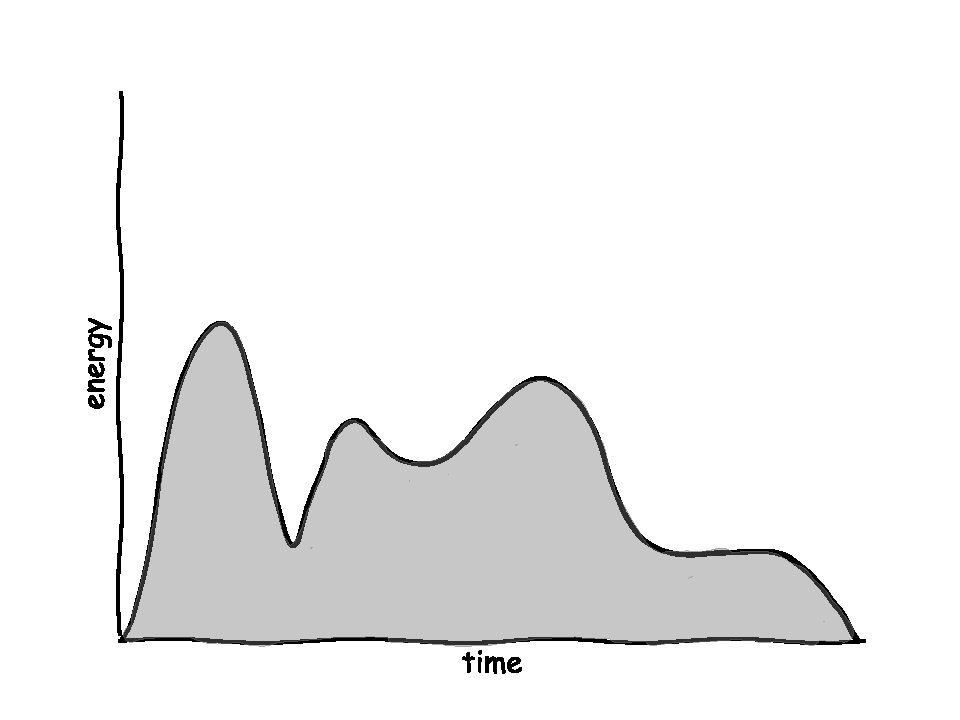
\includegraphics[width=0.5\columnwidth]{plots/Figure_2_demand}%
\caption{This is an example figure. It shows a fictional demand of energy (in grey) over time.}%
\label{fig:example}%
\end{figure}

\section{The GEFCom2014 Dataset}
\label{sec:gefcom-dataset}

In order to compare different energy forecasting methods, 
\Textcite{Hong2016} organized the Global Energy Forecasting Competition 2014 (GEFCom2014), 
a probabilistic energy forecasting competition with four tracks: 
electric load, electric price, wind power and solar power forecasting. 
The competition attracted 581 participants from 61 countries. 

The Global Energy Forecasting Competition took place the first time in 2012. 
In the 2014 competition, they upgraded the competition with three features: 
\begin{enumerate}
    \item instead of point forecasts, probabilistic forecasts were used;
    \item four forecasting tracks were used: electric load (L track), 
    electric price (P track), wind power (W track) and solar power (S track);
    \item incremental data releases on a weekly basis to mimic real world forecasting.
\end{enumerate}

In this thesis, we will only look at the solar power track. 
In this track, the task is to predict the power generation of three 
solar power plants (the so called zones) in Australia. 
The prediction is on a rolling basis for \(\SI{24}{\hour}\) ahead. 
The forecasts are to be issued at midnight each day for the next \(24\) hours. 
\(15\) tasks are provided for the challenge. In each one, the participants need to 
provide one month of forecasts, so \(28\)-\(31\) days.
For the forecasts, different prediction variables from the 
European Centre for Medium-Range Weather Forecasts (ECMWF) are provided. 
They are shown in Table \ref{table:predictors}.
Power measurements are also provided, but only over the training period. 

In order to become familiar with the data, only the last twelve of the 15 available tasks 
from April 2013 to June 2014 counted towards the final score.
The final score was calculated using a linear increasing weighted mean over the scores from the different tasks: 
The first task got weight \(1/78\), the second \(2/78\), etc. 
in order to promote models that improve over time. The division by \(78\) is so that the 
weights sum to \(1\).
Since we will evaluate the models on the dataset as a whole instead of on a monthly different basis, 
we will take the mean over the \(12\) different losses.

\begin{table}[ht]
\caption[Predictors for the GEFCom2014-S track]{Predictors for the GEFCom2014-S track \par Adapted from Table 10 in \cite{Hong2016}}
\label{table:predictors}
\rowcolors{2}{white}{gray!25}
\footnotesize
\begin{tabularx}{\textwidth}{llX}
    \toprule
    \tableheads Variable name & \tableheads Units & \tableheads Comments \\
    \midrule
    Total column liquid water (tclw) & \(\si{\kilo\gram\per\square\metre}\) & Vertical integral of cloud liquid water content \\
    Total column ice water (tciw) & \(\si{\kilo\gram\per\square\metre}\) & Vertical integral of cloud ice water content \\
    Surface pressure (SP) & \(\si{\pascal}\) & \\
    Relative humidity at \(\SI{1000}{\milli\barsi}\) (r) & \(\%\) & Relative humidity is defined with respect to saturation of
                                                                  the mixed phase, i.e., with respect to saturation over ice
                                                                  below \(\SI{-23}{\degreeCelsius}\) and with respect to saturation over water 
                                                                  above \(\SI{0}{\degreeCelsius}\). In the regime in between, a quadratic
                                                                  interpolation is applied. \\
    Total cloud cover (TCC) & \(0\)-\(1\) & TCC derived from model levels using the
                                            model's overlap assumption \\
    \(10\)-metre \(U\) wind component (\(10u\)) & \(\si{\metre\per\second}\) & \\
    \(10\)-metre \(V\) wind component (\(10v\)) & \(\si{\metre\per\second}\) & \\
    \(2\)-metre temperature (\(2T\)) & \(\si{\kelvin}\) & \\
    Surface solar rad down (SSRD) & \(\si{\joule\per\square\metre}\) & Accumulated field \\
    Surface thermal rad down (STRD) & \(\si{\joule\per\square\metre}\) & Accumulated field \\
    Top net solar rad (TSR) & \(\si{\joule\per\square\metre}\) & Net solar radiation at the top of the atmosphere. Accumulated field \\
    Total precipitation (TP) & \(\si{\metre}\) & Convective precipitation \(+\) stratiform precipitation (CP + LSP). Accumulated field \\
    \bottomrule
\end{tabularx}
\end{table}
\chapter{Data}
\label{ch:data}

In this chapter, we introduce the data relevant for this thesis. 
First, we describe the GEFCom2014 competition before explaining  
the data in the competition and the error measure in use. 

\section{The GEFCom2014 Dataset}
\label{sec:gefcom-dataset}

In order to compare different energy forecasting methods, 
\Textcite{Hong2016} organized the Global Energy Forecasting Competition 2014 (GEFCom2014), 
a probabilistic energy forecasting competition with four tracks: 
electric load, electric price, wind power and solar power forecasting. 
The competition attracted 581 participants from 61 countries. 

The Global Energy Forecasting Competition took place the first time in 2012. 
In the 2014 competition, they upgraded the competition with three features: 
\begin{enumerate}
    \item instead of point forecasts, probabilistic forecasts were used;
    \item four forecasting tracks were used: electric load (L track), 
    electric price (P track), wind power (W track) and solar power (S track);
    \item incremental data releases on a weekly basis to mimic real world forecasting.
\end{enumerate}

In this thesis, we will only look at the solar power track. 
In this track, the task is to predict the power generation of three 
solar power plants (the so called zones) in Australia. 
The prediction is on a rolling basis for \(\SI{24}{\hour}\) ahead. 
The forecasts are to be issued at midnight each day for the next \(24\) hours. 
\(15\) tasks are provided for the challenge. In each one, the participants need to 
provide one month of forecasts, so \(28\)-\(31\) days.
For the forecasts, different prediction variables from the 
European Centre for Medium-Range Weather Forecasts (ECMWF) are provided. 
They are shown in Table \ref{table:predictors}.
Power measurements are also provided, but only over the training period. 

In order to become familiar with the data, only the last twelve of the 15 available tasks 
from April 2013 to June 2014 counted towards the final score.
The final score was calculated using a linear increasing weighted mean over the scores from the different tasks: 
The first task got weight \(1/78\), the second \(2/78\), etc. 
in order to promote models that improve over time. The division by \(78\) is so that the 
weights sum to \(1\).
Since we will evaluate the models on the dataset as a whole instead of on a monthly different basis, 
we will take the mean over the \(12\) different losses.

\begin{table}[ht]
\caption[Predictors for the GEFCom2014-S track]{Predictors for the GEFCom2014-S track \par Adapted from Table 10 in \cite{Hong2016}}
\label{table:predictors}
\rowcolors{2}{white}{gray!25}
\footnotesize
\begin{tabularx}{\textwidth}{llX}
    \toprule
    \tableheads Variable name & \tableheads Units & \tableheads Comments \\
    \midrule
    Total column liquid water (tclw) & \(\si{\kilo\gram\per\square\metre}\) & Vertical integral of cloud liquid water content \\
    Total column ice water (tciw) & \(\si{\kilo\gram\per\square\metre}\) & Vertical integral of cloud ice water content \\
    Surface pressure (SP) & \(\si{\pascal}\) & \\
    Relative humidity at \(\SI{1000}{\milli\barsi}\) (r) & \(\%\) & Relative humidity is defined with respect to saturation of
                                                                  the mixed phase, i.e., with respect to saturation over ice
                                                                  below \(\SI{-23}{\degreeCelsius}\) and with respect to saturation over water 
                                                                  above \(\SI{0}{\degreeCelsius}\). In the regime in between, a quadratic
                                                                  interpolation is applied. \\
    Total cloud cover (TCC) & \(0\)-\(1\) & TCC derived from model levels using the
                                            model's overlap assumption \\
    \(10\)-metre \(U\) wind component (\(10u\)) & \(\si{\metre\per\second}\) & \\
    \(10\)-metre \(V\) wind component (\(10v\)) & \(\si{\metre\per\second}\) & \\
    \(2\)-metre temperature (\(2T\)) & \(\si{\kelvin}\) & \\
    Surface solar rad down (SSRD) & \(\si{\joule\per\square\metre}\) & Accumulated field \\
    Surface thermal rad down (STRD) & \(\si{\joule\per\square\metre}\) & Accumulated field \\
    Top net solar rad (TSR) & \(\si{\joule\per\square\metre}\) & Net solar radiation at the top of the atmosphere. Accumulated field \\
    Total precipitation (TP) & \(\si{\metre}\) & Convective precipitation \(+\) stratiform precipitation (CP + LSP). Accumulated field \\
    \bottomrule
\end{tabularx}
\end{table}
\chapter{Model description}
\label{ch:model-description}

In this chapter, we motivate why the models were selected and 
describe their basic functionality as well as their advantages.

Quantile Random Forests have proven to be a very competitive 
and powerful quantile regression method for high-dimensional datasets. 
There is a lot of literature that discuss which configurations and hyperparameter 
choices function well for Quantile Random Forests. Therefore, they do not only perform 
well but they are also simple to implement as a benchmark.
This is the reason why we use it to compare the other two models 
against it.
Nearest Neighbor Quantile Regression is the method utilized by the first place 
in the GEFCom14 challenge. NNQF uses a similar strategy but requires much less 
computation power in order to predict its output. 
SQF-RNN uses autoregressive input with an RNN structure and provides flexible 
conditional output distributions through spline quantile functions. 
\Textcite{Gasthaus2019} already shows that it works well on large solar energy 
forecasting datasets.

In order to describe the model in the following subsections, we will introduce the necessary notation here:
\begin{itemize}
    \item \(n\) is the training data length
    \item \(x_1, \ldots, x_n \in \R^D\) are the predictor values of the time series
    \item \(y_1, \ldots, y_n \in \R\) are the corresponding target values
\end{itemize}

\section{Quantile Regression Forests}
\label{sec:qrf}

Quantile Regression Forests were first proposed by \Textcite{Meinshausen2006}
and have since then proven to be a powerful method for high-dimensional quantile 
regression and time series forecasting. 
The method works in a similar way as Random Forest with the main difference 
being that we don't take the mean over the trees but take different quantiles 
from the trees.

The performance of this algorithm is very competitive in comparison with other 
linear and tree-based methods.
Therefore, they provide a competitive baseline for this thesis. 

\Textcite{Meinshausen2006} also shows that Quantile Regression Forests are consistent 
under some specific assumptions about the distribution of the covariates, the proportion of observations, the splitting criterion and the 
continuity and monotonicity of the \gls{cdf}.

Quantile Regression Forests work as follows (cf. \Textcite{Meinshausen2006}):
\begin{enumerate}
    \item Grow \(k\) trees \(\func{T_1, \ldots, T_k}{\R^D}{\R}\) like in a Random Forest from the training data.
    \item For a given \(x\in\R^D\), calculate the outputs \( \tilde{y}_i = T_i(x) \) for all \(i \in \set{1, \ldots, k}\).
    \item Calculate the empirical quantiles \(y_{(0.01)}, \ldots, y_{(0.99)}\) from 
    \(\set{\tilde{y}_1, \ldots, \tilde{y}_k}\).
\end{enumerate}

\section{Nearest Neighbor Quantile Filters}
\label{sec:nnqf}

\Textcite{Ordiano2019} proposed a method for probabilistic 
energy forecasting using quantile regression based on a \gls{nnqf}. 
The method works as follows: first, the training set is modified 
by using the Nearest Neigbor Quantile Filters so that 
the training data directly represents a probabilistic distribution. 
Then, a regression model like an artificial neural network can 
train on this modified data set and learn the quantile function.

The preprocessing of the NNQF method includes multiple steps. 
Firstly, we search the \(k\) nearest neighbors 
for every \(x_i\).
The distance metric can be any distance metric on \(\R^D\), 
the euclidean metric is used often.
Let \(J \subset \set{1, \ldots, n}\) be the indices of 
those nearest neighbors. 
The probabilistic distribution of \(y_i\) can be approximated 
by calculating the empirical quantile \(\tilde{y}_{(q),i}\) of 
\(\set{y_j \;|\; j\in J}\) for each \(q \in \set{0.01, \ldots, 0.99}\). 

After repeating this procedure for each entry in the time series, 
we get vectors 
\[ \tilde{y}_{(q)} = \begin{pmatrix}
    \tilde{y}_{(q), 1} \\ 
    \vdots \\
    \tilde{y}_{(q), n}
\end{pmatrix} \]
that form the modified training set combined with the 
predictors \(X = (x_1, \ldots, x_n)\).

Because we work with a time series, adjacent points are correlated. 
That's the reason why we use lag features: 
instead of only \(x_i\), we are using \(x_i, \ldots, x_{i-H+1}\) to 
predict the target data. \(H\) is called lag size.

With the modified training set, one can now train the regression model 
for each quantile and fit the function 
\[ f_\theta(x_i, \ldots, x_{i-H+1}) = \tilde{y}_{(q), i}. \]
Common examples are polynomial regression or 
artificial neural networks. 

This method has three main advantages: 
\begin{enumerate}
    \item The technique for the quantile regression is not specified, 
    any technique can be used,
    \item the calculation of the nearest neighbors and the modified 
    training set only needs to be done once, you can save time when 
    using multiple quantile regressions. 
    \item The original dataset does not need to be saved afterwards, 
    we only need the weights of the regression model for predicting.
\end{enumerate}

In comparison to most other \(k\)-Nearest Neighbors quantile 
regression techniques, the nearest neighbors are only calculated once 
and then the regression model is trained on the modified training data. 
A regular \(k\)-Nearest Neighbor quantile regression algorithm 
calculates the nearest neighbors every time when a forecast is conducted 
(cf. \Textcite{Ma2015}, p. 3 ff) which is computationally more expensive in the long run.

\section{Spline Quantile Function RNNs}
\label{sec:sqf-rnn}

\Textcite{Gasthaus2019} proposed a method for probabilistic forecasting by modeling 
the quantile function with monotonic regression splines. 
The proposed \gls{sqfrnn} model combines the ability to forecast time series 
from recurrent neural networks which was already done by the DeepAR model from \Textcite{Salinas2017}
with the flexibility of being able to 
model the quantile functions with linear splines. 

Let \(x_1, \ldots, x_n \in \R^D\) be the predictor values and 
\(z_1, \ldots, z_n \in \R\) be the target time series. Also, let \(\Theta\) 
be the model parameters, \(\boldsymbol{h}_t\) the network output of 
time step \(t\) and \(\theta_t\) the parameters of the conditional distribution \(\P(z_t | \theta_t)\).
The model works as follows:
Compute the network output \(\boldsymbol{h}_t = h(\boldsymbol{h}_{t-1}, z_{t-1}, x_t, \Theta)\) 
as well as the parameters \(\theta_t = \theta(\boldsymbol{h}_t, \Theta)\) for the distribution
\(\P(z_t | \theta_t)\). \(h(\cdot)\) is a multi-layer RNN with 
LSTM cells and \(\theta(\cdot)\) is a projection layer. 
The quantiles are then used to calculate the loss and train the model parameters \(\Theta\).
The process is illustrated in Figure \ref{fig:deepar-training}.

\begin{figure}[h]%
    \centering
    \begin{tikzpicture}[yscale=-1,node distance=-\pgflinewidth]
    \tikzset{ReceptorNode/.style={circle, draw=black, fill=lightblue, thick, inner sep=2pt, minimum size=30pt}}
    \tikzset{Placeholder/.style={circle, thick, inner sep=2pt, minimum size=30pt}}
    \tikzset{Connection/.style={->, line width=0.5mm}}
    \newcommand{\mynode}[3]{
        \node[ReceptorNode] (circ-#2) at (#1, 0) {\(\boldsymbol{h}_{#2}\)};
        \node (x-#2) at (#1, 1.5) {\(x_{#2}, y_{#3}\)};
        \node (y-#2) at (#1, -1.5) {\(\P(y_{#2}|\boldsymbol{h}_{#2})\)};

        \draw[Connection] (circ-#2) -- (y-#2);
        \draw[Connection] (x-#2)    -- (circ-#2);
    }
    \newcommand{\placeholder}[2]{
        \node[Placeholder] (circ-#2) at (#1, 0) {\(\cdots\)};
        \node (x-#2) at (#1, 1.5) {};
        \node (y-#2) at (#1, -1.5) {\phantom{\(\P(y_{#2}|\boldsymbol{h}_{#2})\)}};
    }
    \newcommand{\connect}[2]{
        \draw[Connection] (circ-#1) -- (circ-#2);
    }

    % Create nodes
    \mynode{1 * 2.5}{1}{0}
    \onslide<2->{
        \mynode{2 * 2.5}{2}{1}
        \connect{1}{2}    
    }
    \onslide<2->{
        \mynode{3 * 2.5}{3}{2}
        \connect{2}{3}    
    }
    \onslide<3->{
        \placeholder{4 * 2.5}{4}
        \connect{3}{4}
    }
    % Last node is called "n"
    \onslide<4->{
        \mynode{5*2.5}{n}{n-1}
        \connect{4}{n}
    }
\end{tikzpicture}
    \caption{DeepAR Training}%
    \label{fig:deepar-training}%
\end{figure}

For the prediction step, the target time series are not known. 
The known history of the time series \(z_1, \ldots, z_{t_0}\) is fed into the 
model and for \(t > t_0\), samples \(\tilde{z}_t \sim \P(z_t | \theta_t)\) 
are generated and fed back into the model for the next time step.
The process is illustrated in Figure \ref{fig:deepar-predicting}.

\begin{figure}[h]%
    \centering
    \begin{tikzpicture}[yscale=-1,node distance=-\pgflinewidth]
    \tikzset{ReceptorNode/.style={circle, draw=black, fill=lightblue, thick, inner sep=2pt, minimum size=30pt}}
    \tikzset{Placeholder/.style={circle, thick, inner sep=2pt, minimum size=30pt}}
    \tikzset{Connection/.style={->, line width=0.5mm}}
    \newcommand{\mynode}[3]{
        \node[ReceptorNode] (circ-#2) at (#1, 0) {\(\boldsymbol{h}_{#2}\)};
        \node (x-#2) at (#1, 1.5) {\(x_{#2}, z_{#3}\)};
        \node (y-#2) at (#1, -1.5) {\(\P(z_{#2}|\boldsymbol{h}_{#2})\)};

        \draw[Connection] (circ-#2) -- (y-#2);
        \draw[Connection] (x-#2)    -- (circ-#2);
    }
    \newcommand{\mynodewithresult}[3]{
        \node[ReceptorNode] (circ-#2) at (#1, 0) {\(\boldsymbol{h}_{#2}\)};
        \node (x-#2) at (#1, 1.5) {\(x_{#2}, z_{#3}\)};
        \node (y-#2) at (#1, -1.5) {\(\P(z_{#2}|\boldsymbol{h}_{#2})\)};
        \node (z-#2) at (#1, -2.5) {\(\tilde{z}_{#2}\)};

        \draw[Connection] (circ-#2) -- (y-#2);
        \draw[Connection] (x-#2)    -- (circ-#2);
        \draw[Connection] (y-#2)    -- (z-#2);
    }
    \newcommand{\mynodewithresultinputsampled}[3]{
        \node[ReceptorNode] (circ-#2) at (#1, 0) {\(\boldsymbol{h}_{#2}\)};
        \node (x-#2) at (#1, 1.5) {\(x_{#2}, \tilde{z}_{#3}\)};
        \node (y-#2) at (#1, -1.5) {\(\P(z_{#2}|\boldsymbol{h}_{#2})\)};
        \node (z-#2) at (#1, -2.5) {\(\tilde{z}_{#2}\)};

        \draw[Connection] (circ-#2) -- (y-#2);
        \draw[Connection] (x-#2)    -- (circ-#2);
        \draw[Connection] (y-#2)    -- (z-#2);
    }
    \newcommand{\placeholder}[2]{
        \node[Placeholder] (circ-#2) at (#1, 0) {\(\cdots\)};
        \node (x-#2) at (#1, 1.5) {};
        \node[opacity=0] (y-#2) at (#1, -1.5) {\(\P(z_{#2}|h_{#2})\)};
    }
    \newcommand{\connect}[2]{
        \draw[Connection] (y-#1)    -- (circ-#2);
        \draw[Connection] (circ-#1) -- (circ-#2);
    }

    % Create nodes
    \mynode{1 * 2.5}{T}{T-1}
    \draw[Connection] ([xshift=-0.5cm]circ-T.west) -- (circ-T);
    \onslide<2->{
        \mynodewithresult{2 * 2.5}{T+1}{T}
        \connect{T}{T+1}
    }
    \onslide<3->{
        \mynodewithresultinputsampled{3 * 2.5}{T+2}{T+1}
        \connect{T+1}{T+2}
    }
    \onslide<4->{
        \placeholder{4 * 2.5}{T+3}
        \connect{T+2}{T+3}
    }
    % Last node is called "T+n"
    \onslide<5->{
        \mynodewithresultinputsampled{5*2.5}{T+n}{T+n-1}
        \connect{T+3}{T+n}
    }
\end{tikzpicture}
    \caption{DeepAR Predicting}%
    \label{fig:deepar-predicting}%
\end{figure}

While the DeepAR model is trained by maximizing the likelihood function, 
the SQF-RNN model is trained by minimizing the CRPS (see \ref{ch:crps}) 
which can be computed effectively for spline-based quantile functions.

A linear spline with \(L\) pieces is of the form 
\[ s(x; \gamma, b, d) = \gamma + \sum_{l=0}^L b_l (x - d_l)_+, 
\quad b, d \in \R^{L+1}. \]
Since we want a monotone spline, we need to create constraints for \(b_l\) and \(d_l\).
We want \(d_l < d_{l+1}\) for ordered knot positions. To achieve this 
in the neural network, we set \(d_0 = 0\) and \(d_l = \sum_{j=1}^l \delta_j\), 
where \(\delta_j \geq 0\) and \(\sum_{j=1}^L \delta_j = 1\) since the domain 
of the quantile function is \([0, 1]\). 
We also want monotonicity: the slope \(m_l\) between two knots is given by 
\(m_l = \sum_{j=0}^l b_j\). We need to make sure that \(m_l \geq 0 \forall l\).
If we set \(b_l = \beta_l - \beta_{l-1}\) and \(b_0 = \beta_0\) with \(\beta_l \geq 0 \forall l\), 
we get \(m_l = \sum_{j=0}^l b_j = \beta_l \geq 0\).
We can therefore model our spline with the parameter 
\(\theta = (\gamma, \beta, \delta)\), \(\gamma \in \R, \beta \in [0,\infty)^{L}, 
\delta \in \set{ \delta \in [0,1]^L: \sum_{j=1}^L \delta_j = 1 }\).
\chapter{Model implementation}
\label{ch:model-implementation}

From all predictors in Table \ref{table:predictors}, only SSRD, STRD, TSR, TP and TCC are used. 
Since the Variables SSRD, STRD and TSR are all available as accumulated fields, they first need to be decumulated.
This can be done by subtracting the value before the current value from the current value, for each day separately. 
Figure \ref{fig:strd-accumulated-vs-decumulated} shows both the accumulated and decumulated fields. 
A machine learning algorithm works better with the decumulated field since the decumulated field directly correlates 
with the power output of the solar plant.

\begin{figure}[h]%
    \centering
    \subfloat[\centering STRD accumulated]{{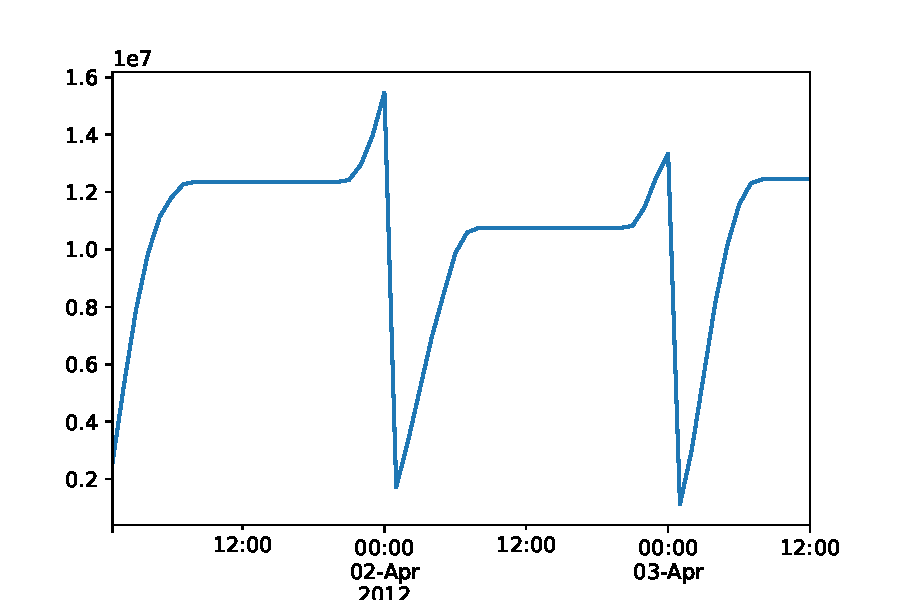
\includegraphics[width=7cm]{plots/strd_accumulated.pdf} }}%
    \qquad
    \subfloat[\centering STRD decumulated]{{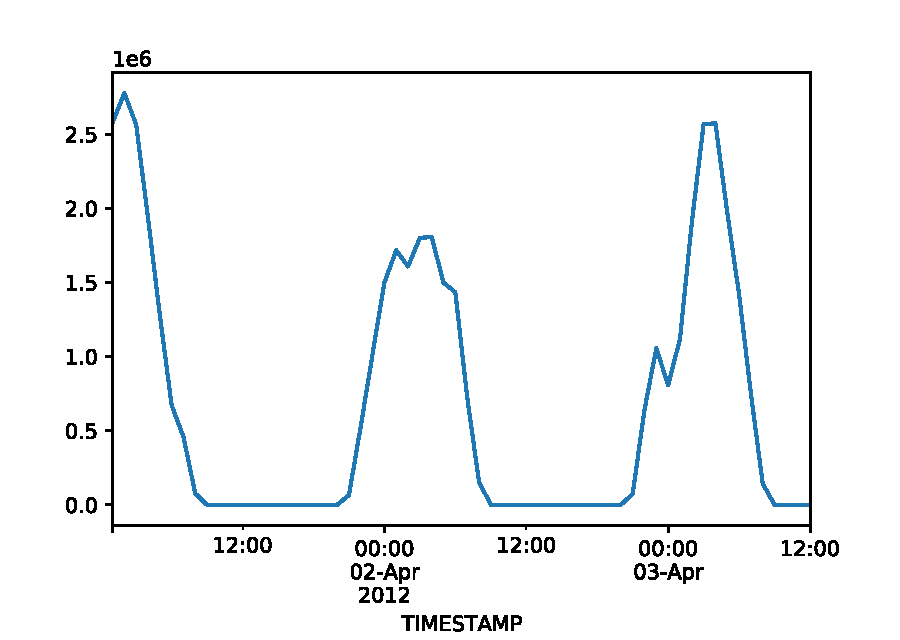
\includegraphics[width=7cm]{plots/strd_decumulated.pdf} }}%
    \caption{STRD accumulated vs. decumulated}%
    \label{fig:strd-accumulated-vs-decumulated}%
\end{figure}

Since we are using some steps like the calculation of the pinball loss, 
it makes sense to use some kind of pipeline structure for the code. 
\Textcite{Heidrich2021} introduced 
pyWATTS\footnote{\url{https://github.com/KIT-IAI/pyWATTS}}: a framework 
that is designed to solve the issue of creating pipelines for time series 
forecasting. 

\section{Spline Quantile Function RNNs}
\label{sec:implementation-sqf-rnn}

The implementation for the SQF-RNN model can be found on GitHub\footnote{\url{https://github.com/awslabs/gluon-ts}}.

The key difference between the SQF-RNN model and the DeepAR model from 
\Textcite{Salinas2017} is that the DeepAR implementation uses a 
probabilistic distribution and optimizes the likelihood of that distribution 
where in the SQF-RNN case spline quantile functions are used and the 
CRPS is optimized. 
For complex problems, the specification on a probabilistic distribution 
that fits the data is often not trivial. 

In the DeepAR default implementation, the Student's \(t\)-distribution is used. 
With this assumption, the model performs noticably worse on the GEFCom14 dataset.

The CRPS is often used to evaluate a forecast model but its usage as 
a direct loss function in the training process is rare. 
As the CRPS is closely related to the pinball loss (see \ref{ch:crps}), 
this helps in the GEFCom14 problem since it directly minimizes the given metric.

First, the data is read from the \texttt{.csv} files. 
After that, the cumulated columns (SSRD, STRD, TSR) are decumulated and then normalized.
Then, the trainig data is converted into a \texttt{ListDataset} and fitted with the 
\texttt{DeepAREstimator} class. The frequency of the model was set to one hour and 
prediction length to 28, 30 or 31 days since the task was to predict one full month. 
In order to use quantile splines with three parts as the output distribution, 
we need to set \texttt{distr\_output=PiecewiseLinearOutput(num\_pieces=3)}. 
Because the default value of \texttt{use\_feat\_dynamic\_real} is set to \texttt{False} 
in the \texttt{DeepAREstimator} model, 
we need to change it to \texttt{True} or else it will ignore the predictors 
\(x_1, \ldots, x_n \in \R^D\). 

After training for seven epochs, the model with the data that is available from the months before, 
we need to predict the upcoming month. This is done by calling the \texttt{predict()} 
method from the predictor that we got after training.
After that, we calculate the quantiles from the prediction and use them to 
calculate the pinball loss for each time step and zone.

In order to get better and more consistent results, the ensemble averaging is used. 
Seven independent models are trained simultaneously and in the predcition step, 
the output of every model is averaged and returned.
\todo{how much performance improvement?}

\section{Nearest Neighbor Quantile Filters}
\label{sec:implementation-nnqf}

The basic steps for the quantile filters are provided by \Textcite{Ordiano2019} 
on GitHub\footnote{\url{https://github.com/JorgeAngel/nnqf_filter}}. 

Since the NNQF method is only a preprocessing step for the target values, 
we still need to decide which model we want to use for fitting the 
conditional distribution function. 
\Textcite{Ordiano2019} tried fitting each of the \(99\) quantiles 
with a polynomial of maximum degree \(1\) to \(4\) or a multi layer perceptron 
with \(6\) or \(10\) hidden neurons. Since the multi layer perceptron leads to 
noticably better results, we will focus on this regression method. 

Because the data is a time series, timepoints that are close are correlated. 
Therefore, we not only take the predictor value \(x_n \in \R^D\) of time point \(n\) 
but also \(x_{n-1}, \ldots, x_{n-H+1}\) as predictor values, where \(H\) is the number of lags.
All in all, we want to fit a function \(\func{f_q}{\R^{D\times H}}{\R}\), 
where \( f(x_n, \ldots, x_{n-H+1}; \theta_{(q)})\) is the conditional 
\(q\)-quantile of the target value \(Y_n\) and \(\theta_{(q)}\) are the weights 
of the regression model for the \(q\)-quantile.

In order to achieve this lagging, pyWATTS contains a \texttt{Sampler} class
that transforms the data in a way that afterwards, each timepoint contains the 
predictor data of the previous \(H\) timepoints.

\Textcite{Ordiano2019} use separate neural networks with \(6\) or \(10\) hidden nodes for each quantile, 
which is computationally more expensive than training one neural network with 
one hidden layer with \(50\) nodes for \(99\) outputs. 
\todo{Both methods perform approximately the same in evaluation chapter; add numbers to show that} 

Since implementing a model in pyWATTS with a variable number of neural networks is currently 
not easily possible, we will use a single neural network to approximate the quantiles.

In order to avoid quantile crossing, \Textcite{Ordiano2019} postprocess the conditional quantiles:
\[ \hat{y}_{(q)} = \begin{cases}
    \max\set{ f(x; \theta_{(q)}), 0 }, &\text{if } q = 0.01, \\
    \max\set{ f(x; \theta_{(q)}), f(x; \theta_{(q-0.01)}) }, &\text{else.}
\end{cases}\]

In this thesis, we use another approach: \\
We sort all estimated conditional quantiles \(\set{ f(x; \theta_{(q)}) \;|\; q\in \set{0.01, \ldots, 0.99} }\) 
and set \(\hat{y}_{(q)}\) as the \((q\cdot 100)\)-th entry of the sorted list. 
\todo{This results in a noticable performance improvement 
in comparison to taking the maximum. add numbers to show noticable improvement! \(\leadsto\) in evaluation chapter}

After that, the pinball loss is calculated the same way as in the QRF case.

In the NNQF model, the only hyperparameters for the preprocessing part are 
the metric that is used calculating the distances, 
the number of neighbors that should be considered and 
the number of lags \(H\). 
The other hyperparameters depend on the regression model. 
In the case of the multi layer perceptron, the usual hyperparameters like 
hidden layer sizes, activation function, solver and learning rate can be tuned. 
To improve stability, we also use ensemble training at the expense of training and evaluation time.
The parameters after tuning as well as the hyperparameter space 
are shown in Table \ref{table:nnqf-hyperparameters}. 
The resulting losses are all in the range \([0.02, 0.025]\) 
but the best loss was already approximately achieved by the default configuration. 
No noticable performance improvement is visible.

\begin{table}[ht]%
    \caption{NNQF Hyperparameters}
    \label{table:nnqf-hyperparameters}
    \rowcolors{2}{white}{gray!25}
    \centering
    \footnotesize
    \begin{tabular}{lll}
    \toprule \noalign{\smallskip}
    \tableheads Hyperparameter & \tableheads Optimization space & \tableheads Value \\ 
    \midrule
    Number of neighbors & \(\set{50, 100, 150, 200}\)     & \(50\)                      \\
    Distance metric     & --                              & euclidean \(|| \cdot ||_2\) \\
    Number of lags      & \(\set{12, 24, 48, 96}\)        & \(12\)                      \\
    Hidden layer sizes  & \(\set{(50), (50, 50), (100), 
                          (50, 100, 50)}\)                & one layer with \(50\) nodes \\
    Activation function & \(\set{\text{ReLU}, \tanh}\)    & ReLU                        \\
    Solver              & --                              & Adam                        \\
    Learning rate       & \(\set{0.0001,0.001,0.01,0.1}\) & \(0.001\)                   \\
    Ensemble size       & --                              & \(3\)                       \\
    \bottomrule
    \end{tabular}
\end{table}

\section{Quantile Regression Forests}
\label{sec:implementation-qrf}

A Python implementation for Quantile Regression Forests can 
be found in the doubt package\footnote{\url{https://github.com/saattrupdan/doubt}}.

First, the data is read from the \texttt{.csv} files. 
Afterwards, the cumulated columns (SSRD, STRD, TSR) are decumulated and then normalized 
as described in Section \ref{sec:data-preprocessing}.
Then, the \texttt{QuantileRegressionForest} is wrapped into a pipeline stage in order for 
it to be trained.
After training and prediction, the results are evaluated 
using the pinball loss scoring rule for each time step and zone.

The hyperparameters of Quantile Regression Forests are very similar to the ones 
of conventional Random Forests. We can choose the number of trees in the forest, 
the splitting criterion (mean squared error or mean absolute error), 
the splitting strategy (best split or best random split) 
and the number of features to consider when looking for the best split. 
We can also change the shape of the trees: 
the maximum depth, minimum number of samples required to split a node, the minimum number of samples per leaf and 
the maximum number of leaf nodes can all be adjusted.
The parameters after tuning as well as the optimization space 
are shown in Table \ref{table:qrf-hyperparameters}; the dash indicates that we don't optimize over this value.
Most of the losses are in the range \([0.18, 0.24]\). 
The default configuration resulted in a loss of \(0.2\) so 
the optimization results in an improvement of around \(10\%\).

\begin{table}[h!]%
    \caption{QRF Hyperparameters}
    \label{table:qrf-hyperparameters}
    \rowcolors{2}{white}{gray!25}
    \centering
    \footnotesize
    \begin{tabular}{lll}
    \toprule \noalign{\smallskip}
    \tableheads Hyperparameter & \tableheads Optimization space & \tableheads Final value \\ 
    \midrule
    Number of trees                             & \(\set{50, 100, 150, 200}\)    & \(100\)            \\
    Splitting criterion                         & --                             & mean squared error \\
    Splitting strategy                          & --                             & best split         \\
    Maximum number of features for split        & \(\set{1, 2, 3, 
                                                  \text{number of features}}\)   & \(3\)              \\
    Maximum depth                               & \(\set{5, 10, 20, 30, 40, 50, 
                                                  \text{any size}}\)             & \(10\)             \\
    Minimum number of samples required to split & \(\set{2, 4, 6, 8, 10}\)       & \(4\)              \\
    Minimum number of samples per leaf          & \(\set{1, 2, 4, 8}\)           & \(8\)              \\
    Maximum number of leaves                    & \(\set{50, 100, 200, 300, n}\) & \(50\)             \\
    \bottomrule
    \end{tabular}
\end{table}
\chapter{Evaluation}
\label{ch:Evaluation}

In this chapter, we will look at the results of the different models. 
We first evaluate which features are most important for the models using 
permutation feature importance, then we will look at the pinball scores from 
that are used in the competition. Finally, we will look at how the models performed 
considering another scoring function, the Energy score.

\section{Feature importance}
\label{sec:feature-importance}

One way to determine the importance of a feature for a model is called 
permutation feature importance. Here, the model is trained like usual but for the prediction 
step, we don't use the normal test data, but a modified dataset where one feature is 
shuffled. Like that, the model cannot use the information of this feature properly 
and will most likely perform worse. The performance on the shuffled dataset is 
then divided by the performance on the regular test set. A value close to \(1\) 
indicates that the feature is not that important because the model doesn't perform 
much worse than before. The higher the quotient, the more important the feature is for the model.
Since our time series heavily depends of the time of day, it makes sense 
not to shuffle the whole feature but only the equivalence classes of each hour, 
i.e. the values at \(1\) AM are shuffled, the values at \(2\) AM are shuffled, etc.

Figure \ref{fig:feature-importance} 
shows the results of the permutation feature importance calculation.

\begin{figure}[h!]
    \section{Feature importance}
\label{sec:feature-importance}

One way to determine the importance of a feature for a model is called 
permutation feature importance. Here, the model is trained like usual but for the prediction 
step, we don't use the normal test data, but a modified dataset where one feature is 
shuffled. Like that, the model cannot use the information of this feature properly 
and will most likely perform worse. The performance on the shuffled dataset is 
then divided by the performance on the regular test set. A value close to \(1\) 
indicates that the feature is not that important because the model doesn't perform 
much worse than before. The higher the quotient, the more important the feature is for the model.
Since our time series heavily depends of the time of day, it makes sense 
not to shuffle the whole feature but only the equivalence classes of each hour, 
i.e. the values at \(1\) AM are shuffled, the values at \(2\) AM are shuffled, etc.

Figure \ref{fig:feature-importance} 
shows the results of the permutation feature importance calculation.

\begin{figure}[h!]
    \input{plots/feature_importance}
    \caption[Feature importance]{Feature importance. 
    The table shows the permutation feature importance quotients. 
    The permutation feature importance quotient is 
    the performance of the model with shuffled feature 
    divided by the performance of the model without shuffled features. 
    A higher value indicates a more important feature.}
    \label{fig:feature-importance}
\end{figure}
    \caption[Feature importance]{Feature importance. 
    The table shows the permutation feature importance quotients. 
    The permutation feature importance quotient is 
    the performance of the model with shuffled feature 
    divided by the performance of the model without shuffled features. 
    A higher value indicates a more important feature.}
    \label{fig:feature-importance}
\end{figure}

\section{Pinball Loss}
\label{sec:elaboration-pinball-loss}

As stated in section \ref{sec:pinball-loss-explanation}, the pinball loss is 
used to determine the performance of the different models. 
It is calculated by taking the average over all pinball losses for each time 
point and zone in the dataset. 

Table \ref{table:pinball-loss} and Figure \ref{fig:pinball-loss} show the 
losses of the models for task 4 to task 15 (July 2013 to June 2014). 
We can see that the QRF and NNQF model perform similarly and that the 
SQF-RNN model performs better than the other two during the months from October to Febuary.
Another thing to note is that the DeepAR model always performs worse than the SQF-RNN model.

\begin{table}[ht]%
    \footnotesize
    \hspace*{25pt} % make kind of centering
    \begin{minipage}{\textwidth}
    \renewcommand{\b}[1]{\textbf{#1}}
    \rowcolors{2}{white}{gray!25}
    \begin{tabular}{c|cccccc}
        \toprule \noalign{\smallskip}
        Task & \(4\) & \(5\) & \(6\) & \(7\) & \(8\) & \(9\) \\
        \midrule
        QRF     & \(\b{0.01462}\) & \(\b{0.02022}\) & \(\b{0.01884}\) & \(0.02250\)     & \(0.02258\)     & \(0.02212\)     \\
        NNQF    & \(0.01559\)     & \(0.02091\)     & \(0.01896\)     & \(0.02267\)     & \(0.02330\)     & \(0.02334\)     \\
        SQF-RNN & \(0.02581\)     & \(0.03041\)     & \(0.02451\)     & \(\b{0.01895}\) & \(\b{0.01707}\) & \(\b{0.01833}\) \\
        DeepAR  & \(0.02634\)     & \(0.03649\)     & \(0.02744\)     & \(0.01958\)     & \(0.02579\)     & \(0.02290\)     \\
        \bottomrule
    \end{tabular}
    \vspace*{1em} \\
    \rowcolors{2}{white}{gray!25}
    \begin{tabular}{c|cccccc|c}
        \toprule \noalign{\smallskip}
        Task & \(10\) & \(11\) & \(12\) & \(13\) & \(14\) & \(15\) & Mean \\
        \midrule
        QRF     & \(0.02232\)     & \(\b{0.02012}\) & \(\b{0.01824}\) & \(\b{0.01561}\) & \(\b{0.01355}\) & \(\b{0.01402}\) & \(\b{0.01873}\) \\
        NNQF    & \(0.02333\)     & \(0.02038\)     & \(0.01912\)     & \(0.01673\)     & \(0.01363\)     & \(0.01480\)     & \(0.01940\)     \\
        SQF-RNN & \(\b{0.02002}\) & \(0.02104\)     & \(0.02204\)     & \(0.01684\)     & \(0.01338\)     & \(0.01648\)     & \(0.02041\)     \\
        DeepAR  & \(0.02320\)     & \(0.02612\)     & \(0.02424\)     & \(0.02282\)     & \(0.01865\)     & \(0.01889\)     & \(0.02437\)     \\
        \bottomrule
    \end{tabular}
    \end{minipage}

    \caption[Pinball loss]{Pinball loss. 
    Each task is one month in the training period. 
    Task 4 represents July 2013, Task 5 August 2013, etc. up until June 2014.
    The pinball loss is calculated by averaging 
    over all pinball losses for each time point and zone.}
    \label{table:pinball-loss}
\end{table}

\begin{figure}[ht]
    \centering
    \section{Pinball Loss}
\label{sec:elaboration-pinball-loss}

As stated in section \ref{sec:pinball-loss-explanation}, the pinball loss is 
used to determine the performance of the different models. 
It is calculated by taking the average over all pinball losses for each time 
point and zone in the dataset. 

Table \ref{table:pinball-loss} and Figure \ref{fig:pinball-loss} show the 
losses of the models for task 4 to task 15 (July 2013 to June 2014). 
We can see that the QRF and NNQF model perform similarly and that the 
SQF-RNN model performs better than the other two during the months from October to Febuary.
Another thing to note is that the DeepAR model always performs worse than the SQF-RNN model.

\begin{table}[ht]%
    \footnotesize
    \hspace*{25pt} % make kind of centering
    \begin{minipage}{\textwidth}
    \renewcommand{\b}[1]{\textbf{#1}}
    \rowcolors{2}{white}{gray!25}
    \begin{tabular}{c|cccccc}
        \toprule \noalign{\smallskip}
        Task & \(4\) & \(5\) & \(6\) & \(7\) & \(8\) & \(9\) \\
        \midrule
        QRF     & \(\b{0.01462}\) & \(\b{0.02022}\) & \(\b{0.01884}\) & \(0.02250\)     & \(0.02258\)     & \(0.02212\)     \\
        NNQF    & \(0.01559\)     & \(0.02091\)     & \(0.01896\)     & \(0.02267\)     & \(0.02330\)     & \(0.02334\)     \\
        SQF-RNN & \(0.02581\)     & \(0.03041\)     & \(0.02451\)     & \(\b{0.01895}\) & \(\b{0.01707}\) & \(\b{0.01833}\) \\
        DeepAR  & \(0.02634\)     & \(0.03649\)     & \(0.02744\)     & \(0.01958\)     & \(0.02579\)     & \(0.02290\)     \\
        \bottomrule
    \end{tabular}
    \vspace*{1em} \\
    \rowcolors{2}{white}{gray!25}
    \begin{tabular}{c|cccccc|c}
        \toprule \noalign{\smallskip}
        Task & \(10\) & \(11\) & \(12\) & \(13\) & \(14\) & \(15\) & Mean \\
        \midrule
        QRF     & \(0.02232\)     & \(\b{0.02012}\) & \(\b{0.01824}\) & \(\b{0.01561}\) & \(\b{0.01355}\) & \(\b{0.01402}\) & \(\b{0.01873}\) \\
        NNQF    & \(0.02333\)     & \(0.02038\)     & \(0.01912\)     & \(0.01673\)     & \(0.01363\)     & \(0.01480\)     & \(0.01940\)     \\
        SQF-RNN & \(\b{0.02002}\) & \(0.02104\)     & \(0.02204\)     & \(0.01684\)     & \(0.01338\)     & \(0.01648\)     & \(0.02041\)     \\
        DeepAR  & \(0.02320\)     & \(0.02612\)     & \(0.02424\)     & \(0.02282\)     & \(0.01865\)     & \(0.01889\)     & \(0.02437\)     \\
        \bottomrule
    \end{tabular}
    \end{minipage}

    \caption[Pinball loss]{Pinball loss. 
    Each task is one month in the training period. 
    Task 4 represents July 2013, Task 5 August 2013, etc. up until June 2014.
    The pinball loss is calculated by averaging 
    over all pinball losses for each time point and zone.}
    \label{table:pinball-loss}
\end{table}

\begin{figure}[ht]
    \centering
    \input{plots/pinball_loss}
    \caption[Pinball loss]{Pinball loss. 
    This graph plots the losses of the models for each month of the dataset competition.}
    \label{fig:pinball-loss}
\end{figure}

As described in section \ref{sec:implementation-nnqf}, 
we only use one neural network with more hidden nodes instead of 
separate neural networks for each node. 
The pinball loss for training the model with \(99\) different neural networks 
is \(0.01998\), so the version with one neural network performs approximately the 
same while being noticably faster. 
Another modification to the original algorithm proposed by \Textcite{Ordiano2019} 
is sorting the predicted quantiles instead of taking the maximum as described in 
section \ref{sec:implementation-nnqf}. The avergae pinball loss over all tasks for the second is 
\(0.02742\), so sorting the quantiles instead of taking the maximum of the previous quantile 
results in a noticable performance improvement.
    \caption[Pinball loss]{Pinball loss. 
    This graph plots the losses of the models for each month of the dataset competition.}
    \label{fig:pinball-loss}
\end{figure}

As described in section \ref{sec:implementation-nnqf}, 
we only use one neural network with more hidden nodes instead of 
separate neural networks for each node. 
The pinball loss for training the model with \(99\) different neural networks 
is \(0.01998\), so the version with one neural network performs approximately the 
same while being noticably faster. 
Another modification to the original algorithm proposed by \Textcite{Ordiano2019} 
is sorting the predicted quantiles instead of taking the maximum as described in 
section \ref{sec:implementation-nnqf}. The avergae pinball loss over all tasks for the second is 
\(0.02742\), so sorting the quantiles instead of taking the maximum of the previous quantile 
results in a noticable performance improvement.
\chapter{Discussion and conclusion}
\label{ch:discussion-conclusion}

\section{Discussion}
\label{sec:discussion}

This chapter is supposed to discuss your results. Point out what your results mean.
What are the limitations of your approach, managerial implications or future impact?

Explain the broader picture but be critical with your methods.

\section{Conclusion}
\label{sec:conclusion}

Repeat the problem and its relevance, as well as the contribution (plus quantitative results). 
Look back at what you have written in the introduction.

Provide an outlook for further research steps.

%% --------------------
%% |   Bibliography   |
%% --------------------

%% Add entry to the table of contents for the bibliography
\printbibliography[heading=bibintoc]

%% ----------------
%% |   Appendix   |
%% ----------------
\appendix
%% LaTeX2e class for student theses
%% appendix
%% 
%% Based on SDQ KIT Template by Erik Burger
%%
%% Karlsruhe Institute of Technology
%% Institute for Automation and Applied Informatics
%% AIDA Research Group
%%
%% Nicole Ludwig
%% nicole.ludwig@kit.edu
%%
%% Version 1.2, 2018-10-11


\iflanguage{english}
{\chapter{Appendix}}    % english style
{\chapter{Anhang}}      % german style
\label{ch:appendix}

\section{Proper scoring rules}
\label{sec:proper-scoring-rules}

To measure the error of a probabilistic forecast, one usually uses a 
proper scoring rule. 
Let \(\mathcal{P}\) be a convex class of probability measures on the 
measurable space \((\Omega, \mathcal{A})\).
A \textit{scoring rule} is any extended real-valued function 
\[ \func{S}{\mathcal{P} \times \Omega}{\overline{\R}} \]
such that \(S(P, \cdot)\) is \(\mathcal{P}\)-quasiintegrable for all 
\(P\in \mathcal{P}\).
A scoring rule \(S\) is \textit{proper} relative to a convex subclass 
\(\mathcal{P}_0 \subseteq \mathcal{P}\) if
\[ \int_\Omega S(Q, \omega) \mathrm{d}Q(\omega) \leq \int_\Omega S(P, \omega) \mathrm{d}Q(\omega) \]
for all \(P, Q \in \mathcal{P}_0\). It is \textit{strictly proper} 
if equality holds iff. \(P = Q\).

This property encourages honest and careful quotes by the forecaster. 

\section{CRPS}
\label{ch:crps}

\renewcommand{\d}{\mathrm{d}}

The \gls{crps} is one of the most common 
scoring rules. It is defined as follows: 

\[ \CRPS(F, y) = \int_{-\infty}^\infty \left( F(y) - \mathds{1} \{y \leq x\} \right)^2 \d x, \]
where \(F\) is the CDF of the probabilistic forecast.
We can show that the CRPS can also be written as 
\[ \CRPS(F, y) = 2 \int_0^1 L_\alpha(F^{-1}(\alpha), y) \d \alpha, \]
where \(L_\alpha\) is the pinball loss.
\begin{proof}
    The CRPS can be written as the integral over elementary scoring functions for quantile forecasts: 
    \[ \CRPS(F, y) = 2 \int_0^1 \int_{-\infty}^\infty \mathrm{s}_{\alpha, \eta}(F^{-1}(\alpha), y) \d \eta \d \alpha, \]
    where 
    \[ \mathrm{s}_{\alpha, \eta}(q, y) = \begin{cases}
        1-\alpha, &y\leq \eta < q, \\
        \alpha, &q\leq \eta < y \\
        0, &\text{otherwise}.
    \end{cases} \]

    Let \(\eta < y\). 
    \[ 2 \int_0^1 \mathrm{s}_{\alpha, \eta}(F^{-1}(\alpha), y) \d\alpha = 2 \int_0^{F(\eta)} \alpha \d \alpha = F(\eta)^2 = (F(\eta) - \mathds{1}_{\set{y \leq \eta}})^2. \]
    Let \(\eta \geq y\).
    \[ 2 \int_0^1 \mathrm{s}_{\alpha, \eta}(F^{-1}(\alpha), y) \d\alpha = 2 \int_{F(\eta)}^1 (1-\alpha) \d\alpha = \left[ - (1-\alpha)^2 \right]_{F(\eta)}^1 = (F(\eta) - \mathds{1}_{\set{y \leq \eta}})^2. \]
    Therefore, we get 
    \begin{align*}
        \CRPS(F, y) &= \int_{-\infty}^\infty (F(\eta) - \mathds{1}_{\set{y\leq x}})^2 \d \eta \\
        &= \int_{-\infty}^\infty 2 \int_0^1 \mathrm{s}_{\alpha, \eta}(F^{-1}(\alpha), y) \d \alpha \d \eta \\
        &= 2\int_0^1 \int_{-\infty}^\infty \mathrm{s}_{\alpha, \eta}(F^{-1}(\alpha), y) \d \eta \d \alpha  \tag{Tonelli}.
    \end{align*}
    Thus, we are finished after we conclude \(\int_{-\infty}^\infty \mathrm{s}_{\alpha, \eta}(F^{-1}(\alpha), y) \d \eta = L_\alpha(F^{-1}(\alpha), y)\).

    Let \(F^{-1}(\alpha) < y\). 
    \[ \int_{-\infty}^\infty \mathrm{s}_{\alpha, \eta}(F^{-1}(\alpha), y) \d \eta = \int_{F^{-1}(\alpha)}^y \alpha \d \eta = \alpha (y - F^{-1}(\alpha)) = L_\alpha(F^{-1}(\alpha), y). \]
    Let \(F^{-1}(\alpha) \geq y\). 
    \[ \int_{-\infty}^\infty \mathrm{s}_{\alpha, \eta}(F^{-1}(\alpha), y) \d \eta = \int_y^{F^{-1}(\alpha)} (1-\alpha) \d \eta = (1-\alpha) (F^{-1}(\alpha) - y) = L_\alpha(F^{-1}(\alpha), y). \]
\end{proof}

\section{PIT Histograms}

This section shows the PIT histograms of the different models 
broken down into the predictions for each hour.

\begin{figure}[h]%
    \centering
    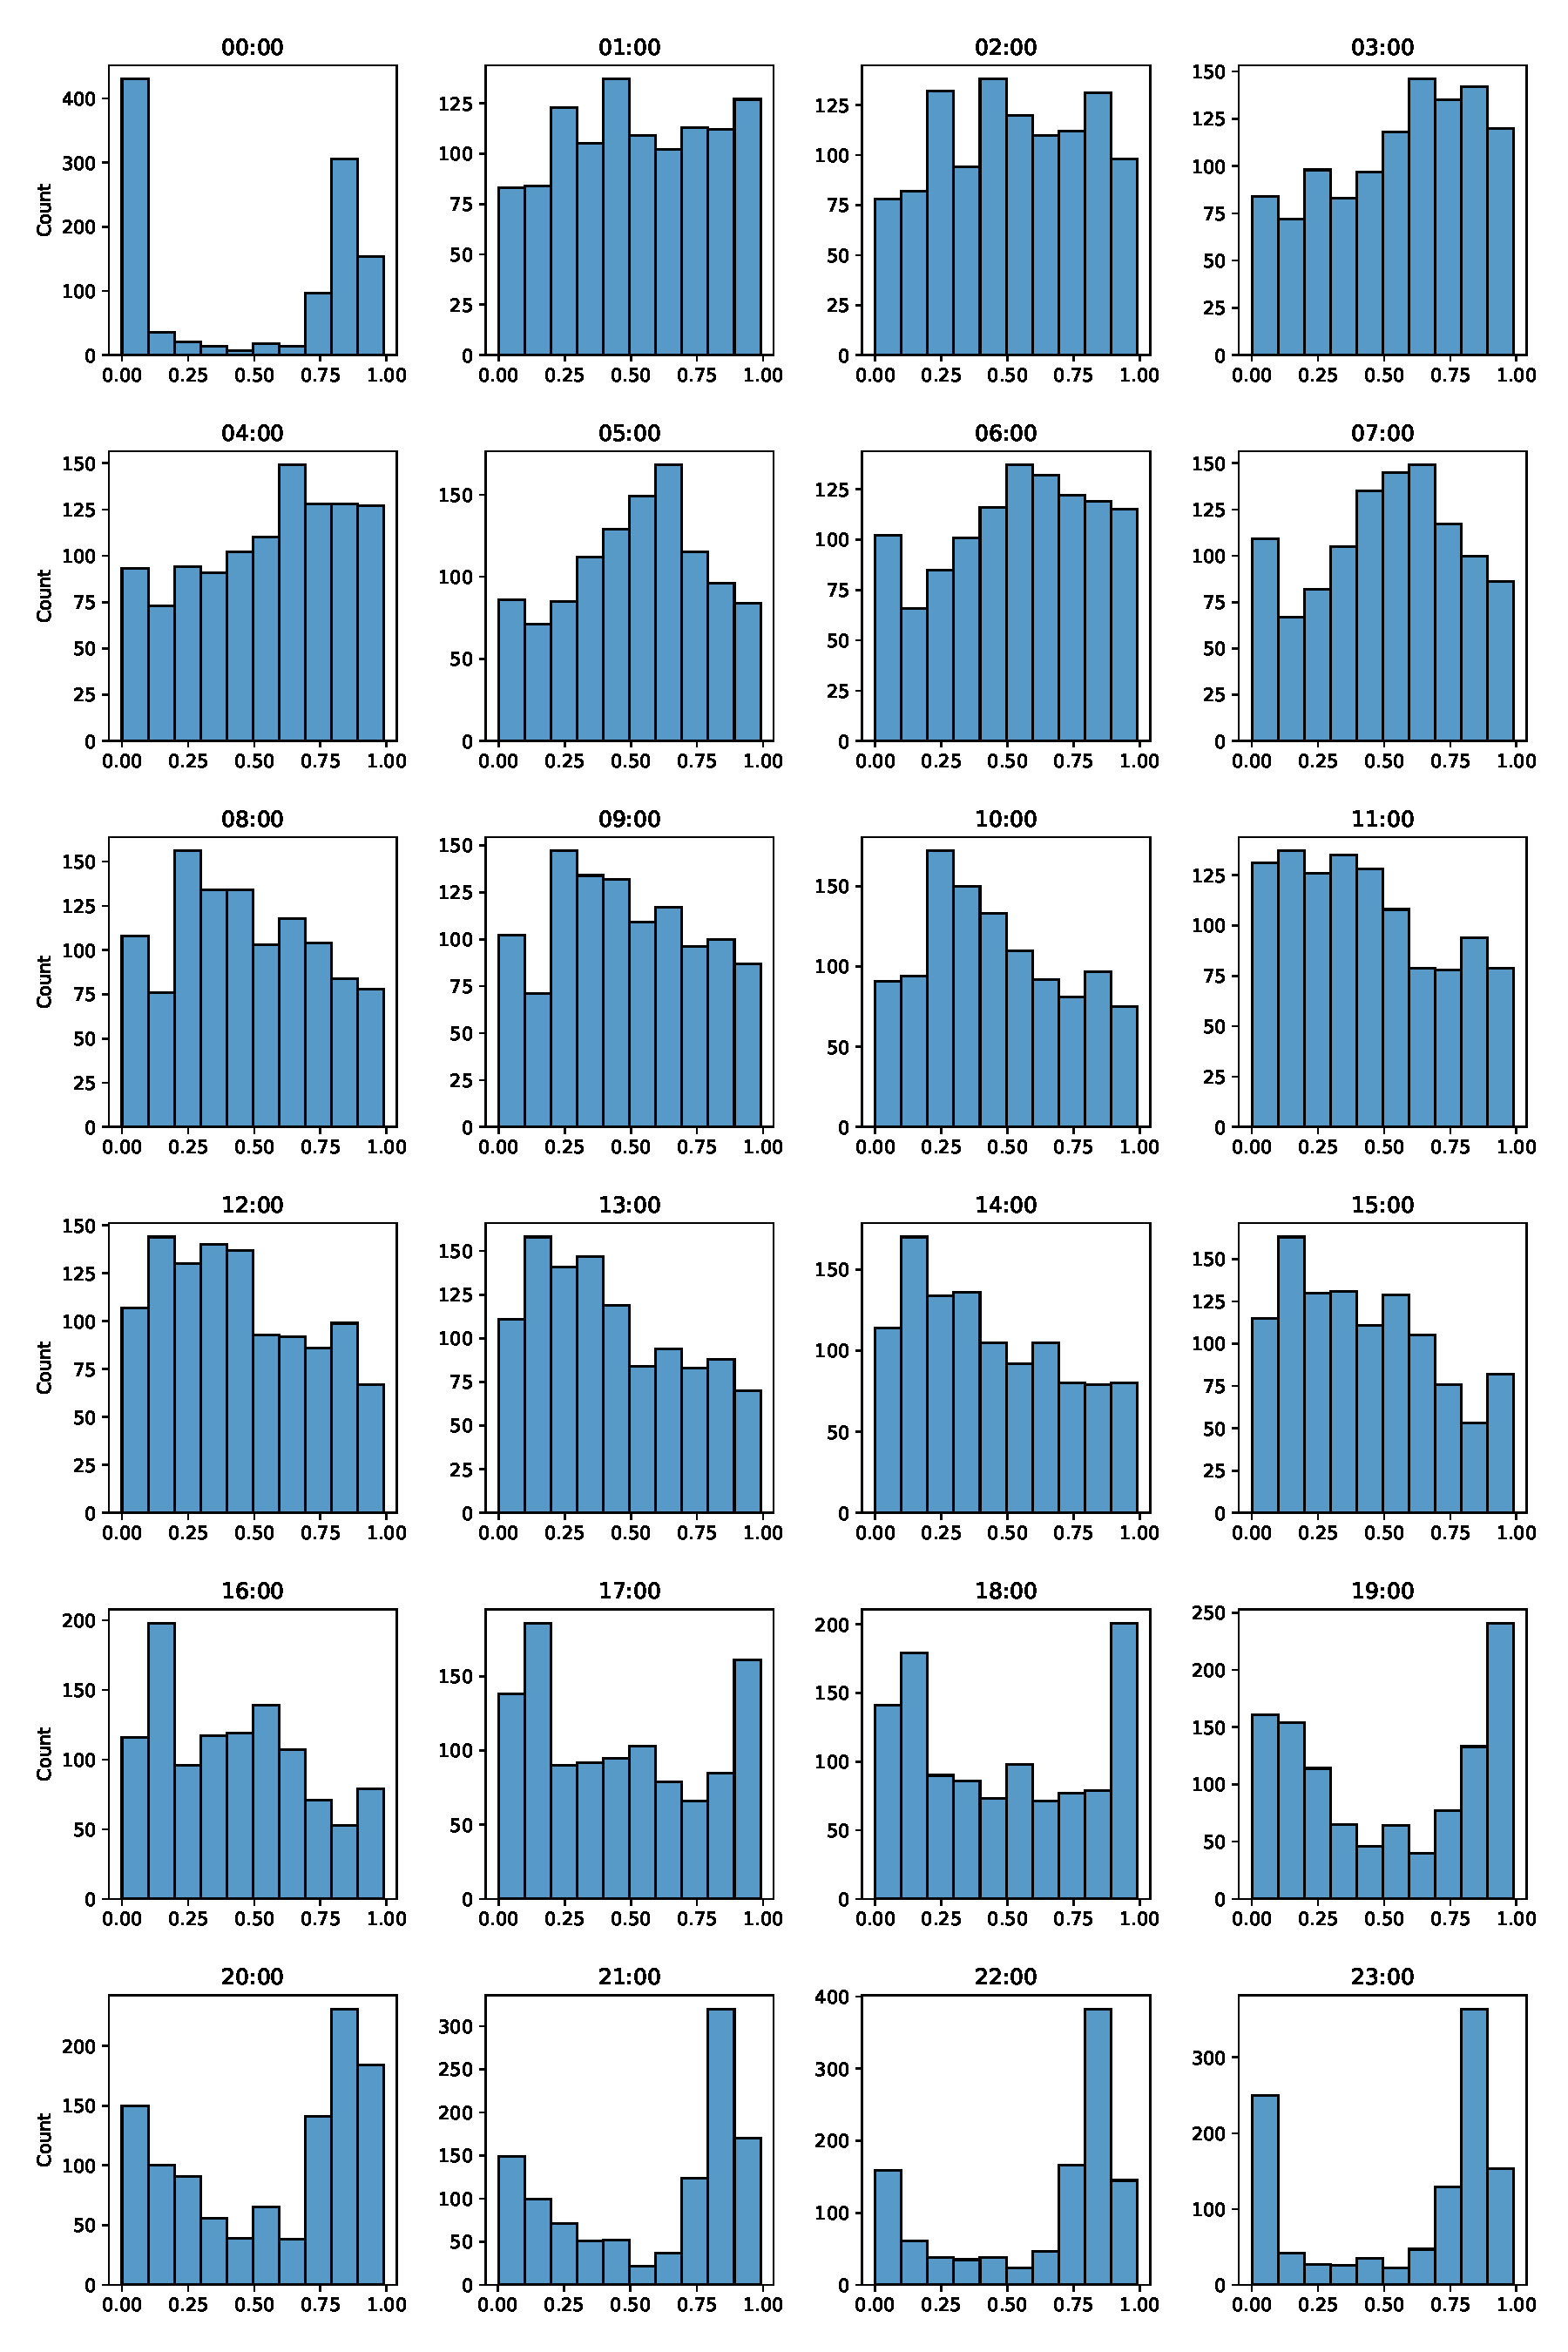
\includegraphics[width=\textwidth]{plots/pit/pit_by_hour_qrf.pdf}
    \caption[PIT histograms QRF]{PIT histograms of QRF. Since the model performs differently 
    in each hour, the PIT histogram is broken down into each hour.}%
    \label{fig:pit-qrf-by-hour}%
\end{figure}

\begin{figure}[h]%
    \centering
    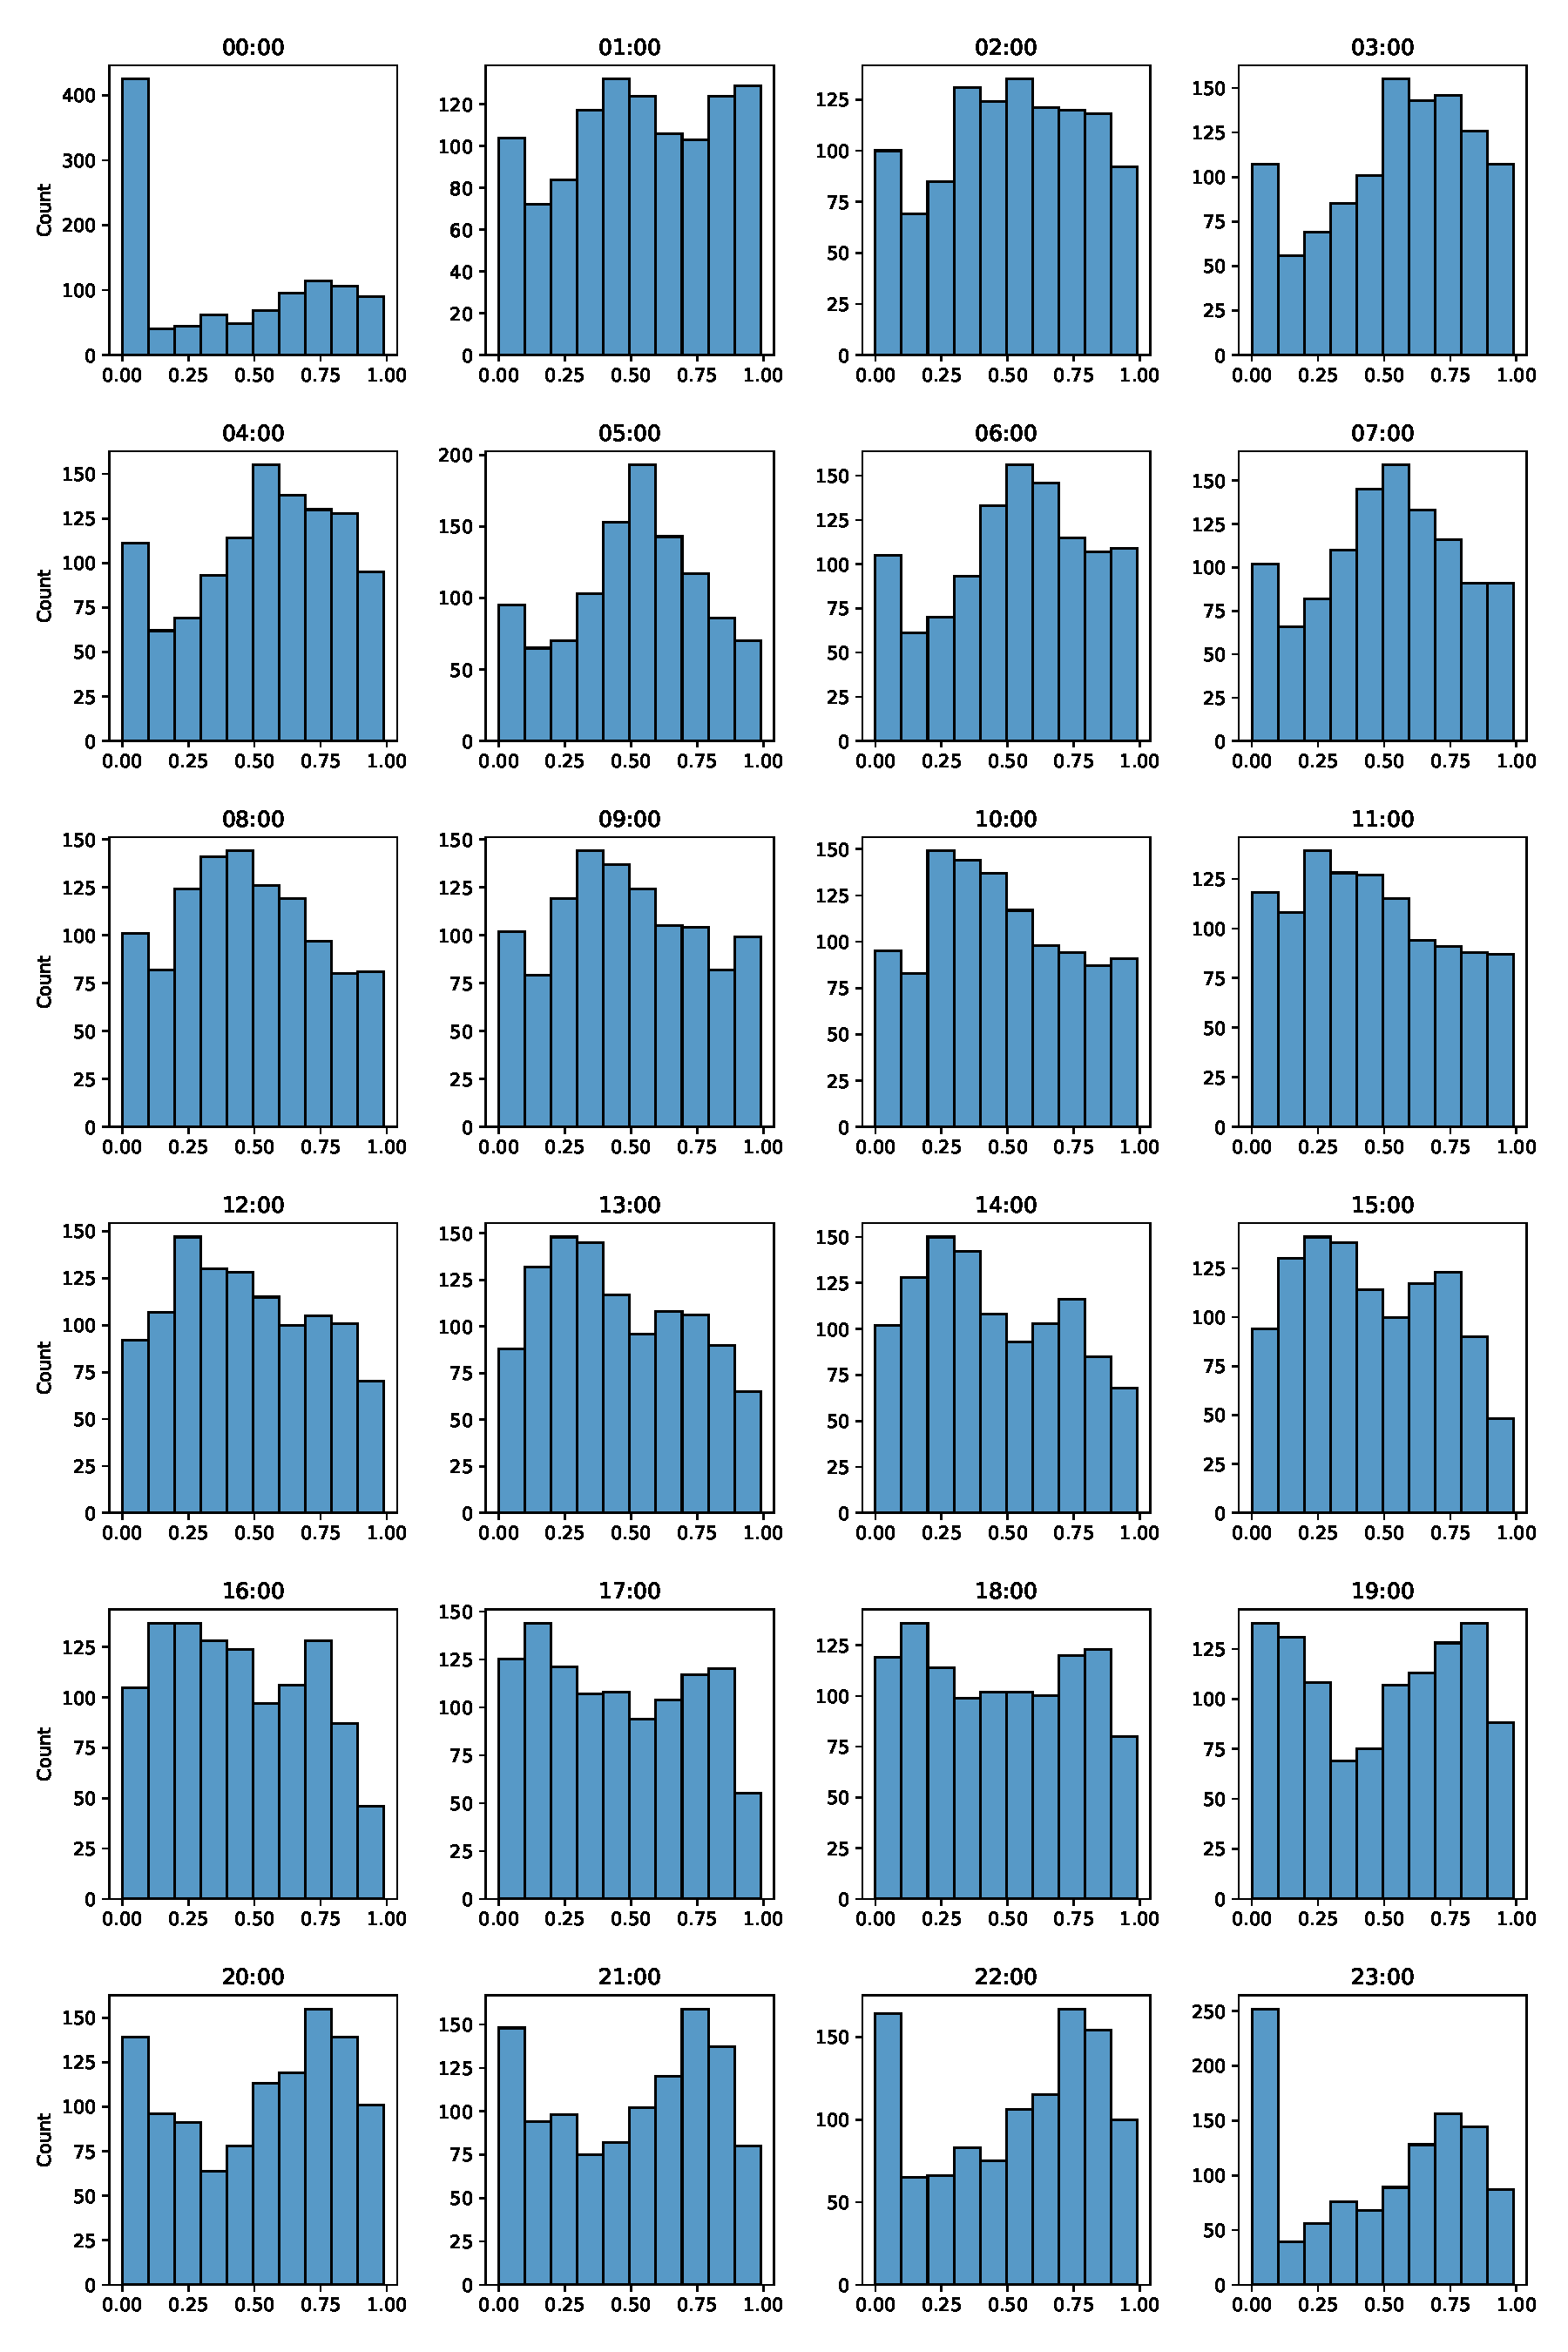
\includegraphics[width=\textwidth]{plots/pit/pit_by_hour_nnqf.pdf}
    \caption[PIT histograms NNQF]{PIT histograms of NNQF. Since the model performs differently 
    in each hour, the PIT histogram is broken down into each hour.}%
    \label{fig:pit-nnqf-by-hour}%
\end{figure}

\begin{figure}[h]%
    \centering
    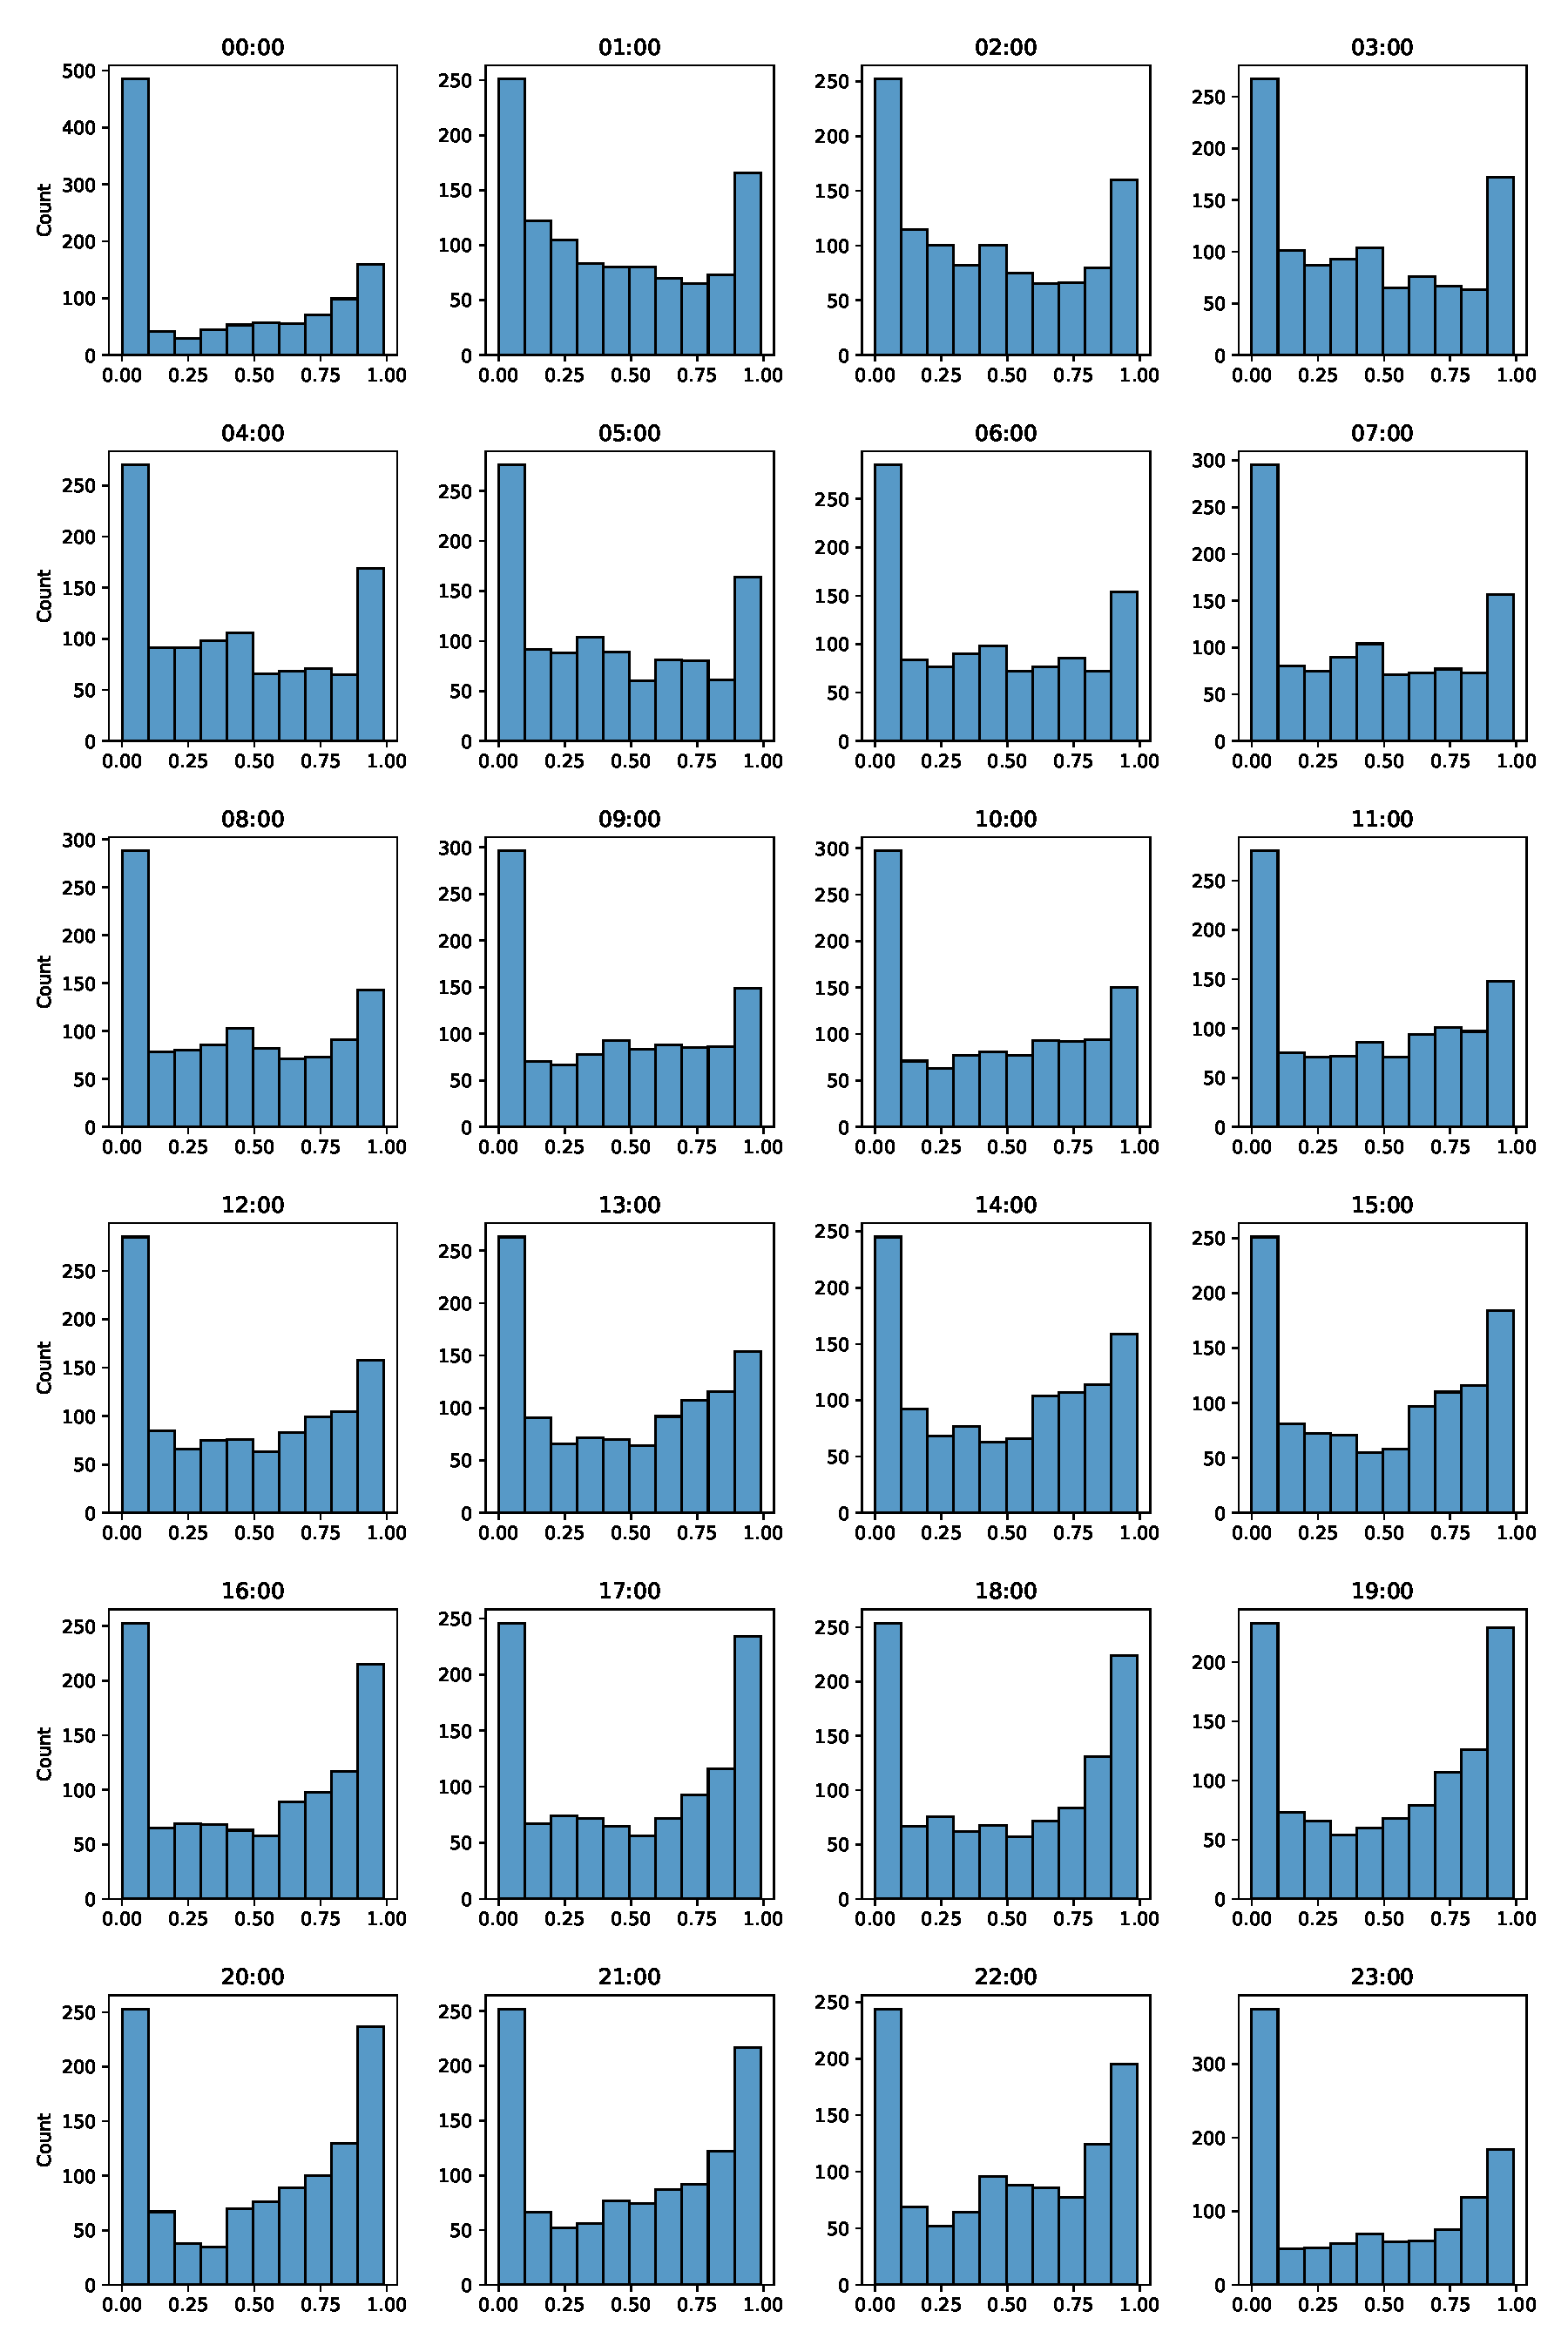
\includegraphics[width=\textwidth]{plots/pit/pit_by_hour_deepar.pdf}
    \caption[PIT histograms DeepAR]{PIT histograms of DeepAR. Since the model performs differently 
    in each hour, the PIT histogram is broken down into each hour.}%
    \label{fig:pit-deepar-by-hour}%
\end{figure}

\begin{figure}[h]%
    \centering
    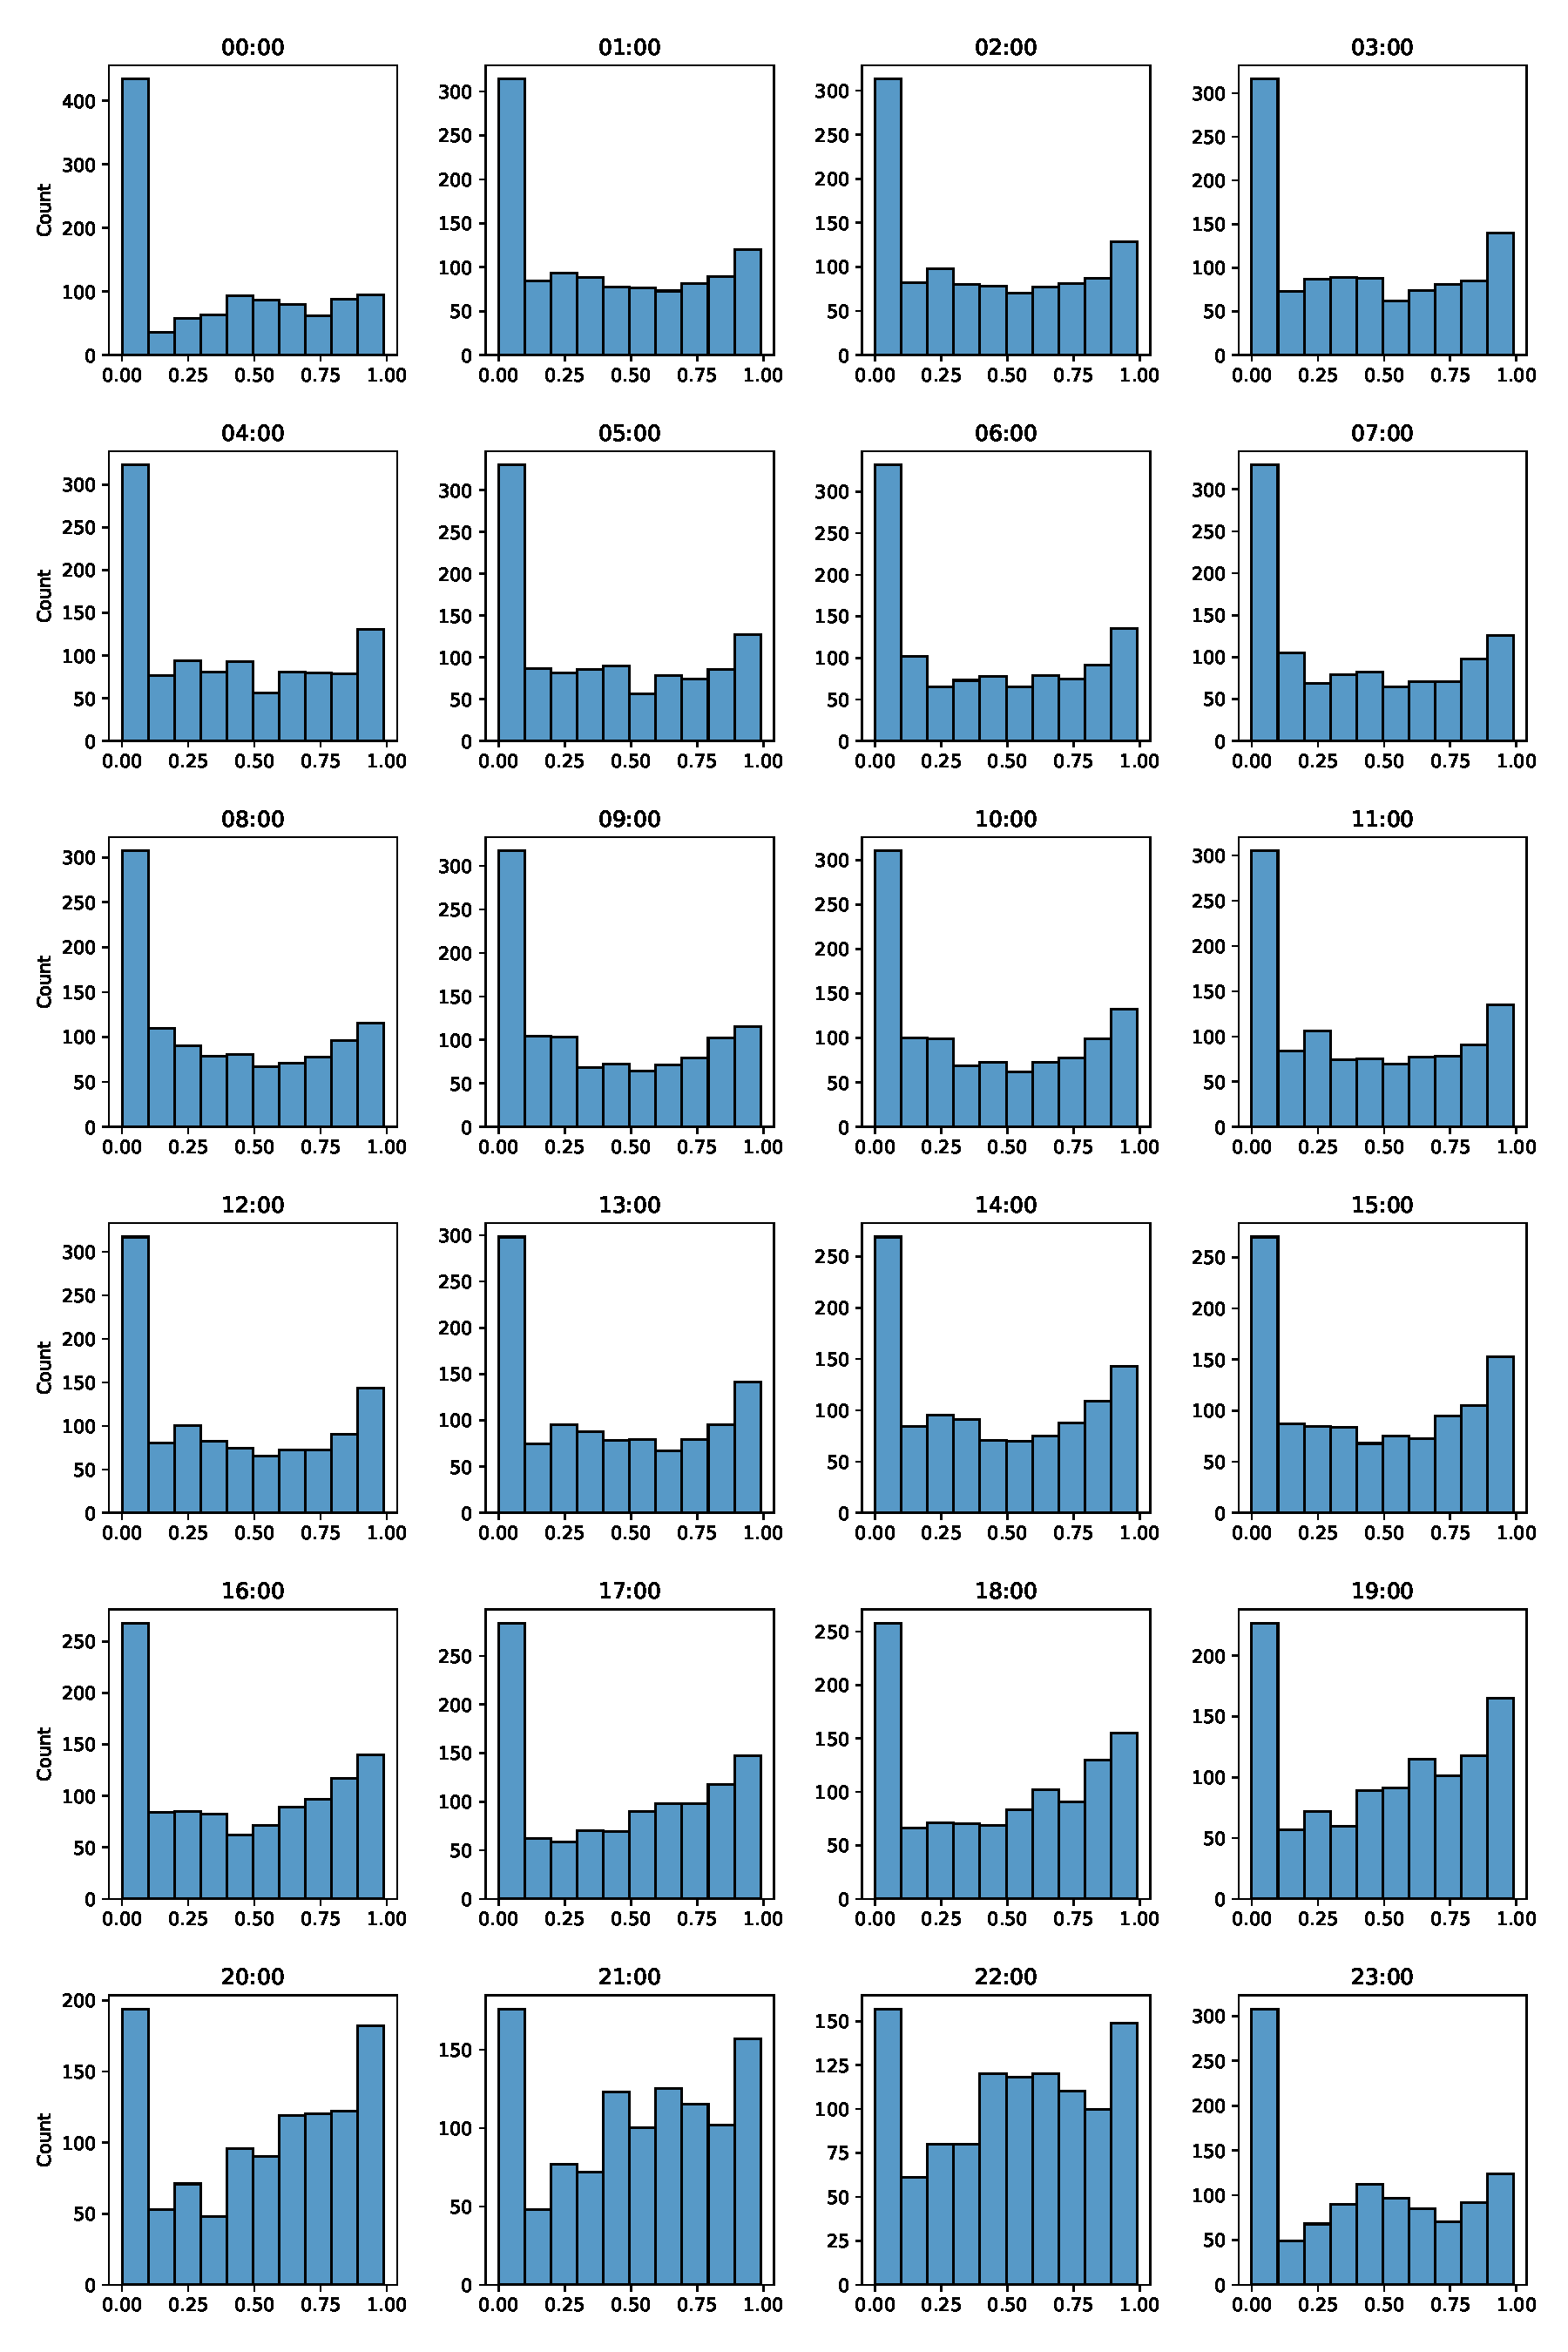
\includegraphics[width=\textwidth]{plots/pit/pit_by_hour_sqf-rnn.pdf}
    \caption[PIT histograms SQF-RNN]{PIT histograms of SQF-RNN. Since the model performs differently 
    in each hour, the PIT histogram is broken down into each hour.}%
    \label{fig:pit-sqf-rnn-by-hour}%
\end{figure}

\end{document}